\chapter{Backend consistency and physical verification}
\label{chap:backend-consistency}

This chapter begins the computational-results part of the report. Its purpose is to establish
that later runtime comparisons refer to physically credible solutions and to the same
resolved numerical solution on each backend. A backend-difference map is meaningful only
when viewed beside the physical field from which it was obtained. Each two-dimensional
case is therefore followed from its resolved evolution and final field to a method-comparison
slice and, finally, the much smaller backend discrepancy. Exact one-dimensional references
and positivity checks complete the verification.

\section{Comparison procedure}

The backend study uses the official HLLC implementations of WENO-2, WENO-3
and ADER-3.  Two resolutions serve different purposes in this chapter.  The
cell-by-cell backend-consistency matrix uses a \(100\times100\) grid, which is
sufficient to expose implementation differences while keeping the full
serial--OpenMP--CUDA matrix manageable.  The resolved physical-field figures
use \(600\times600\) grids so that smooth profiles, contacts and shock-driven
structures are displayed without coarse-grid visualisation error.

For each problem--method pair in the \(100\times100\) consistency matrix, the
complete exported fields from serial, 16-thread OpenMP and CUDA are compared
cell by cell, with serial as the reference.  Maximum absolute backend
differences are evaluated separately for density \(\rho\), velocity components
\(u\) and \(v\), pressure \(p\), and total-energy density \(E\). The largest of
these five discrepancies is reported below.  These are backend-consistency
differences, not errors relative to an exact solution.  The same check verifies
that every exported value is finite and records the minimum density and
pressure for the admissibility assessment.

The CFL values follow the stable method-specific policy established in
Chapter~\ref{chap:methodology}.  Smooth WENO-2 and WENO-3 use CFL \(0.40\),
whereas smooth ADER-3 uses \(0.25\).  For both discontinuous problems, the
WENO methods use CFL \(0.20\) and ADER-3 uses \(0.14\).  Within each
problem--method comparison, all three backends use the same grid, CFL,
final time, initial and boundary conditions, and time-step formula. Only
the execution backend changes.

\section{One-dimensional physical verification}

\subsection*{Continuous advection}

The one-dimensional evidence begins with periodic sinusoidal and Gaussian advection.
These two profiles test complementary aspects of smooth transport: the sinusoid exposes
phase and amplitude errors across the full domain, whereas the compact Gaussian exposes
peak damping and broadening. Figure~\ref{fig:continuous-1d-fields} compares all three
methods with exact cell-average references at \(n=800\).

\begin{figure}[!htbp]
\centering
\begin{subfigure}[t]{0.49\textwidth}
\centering
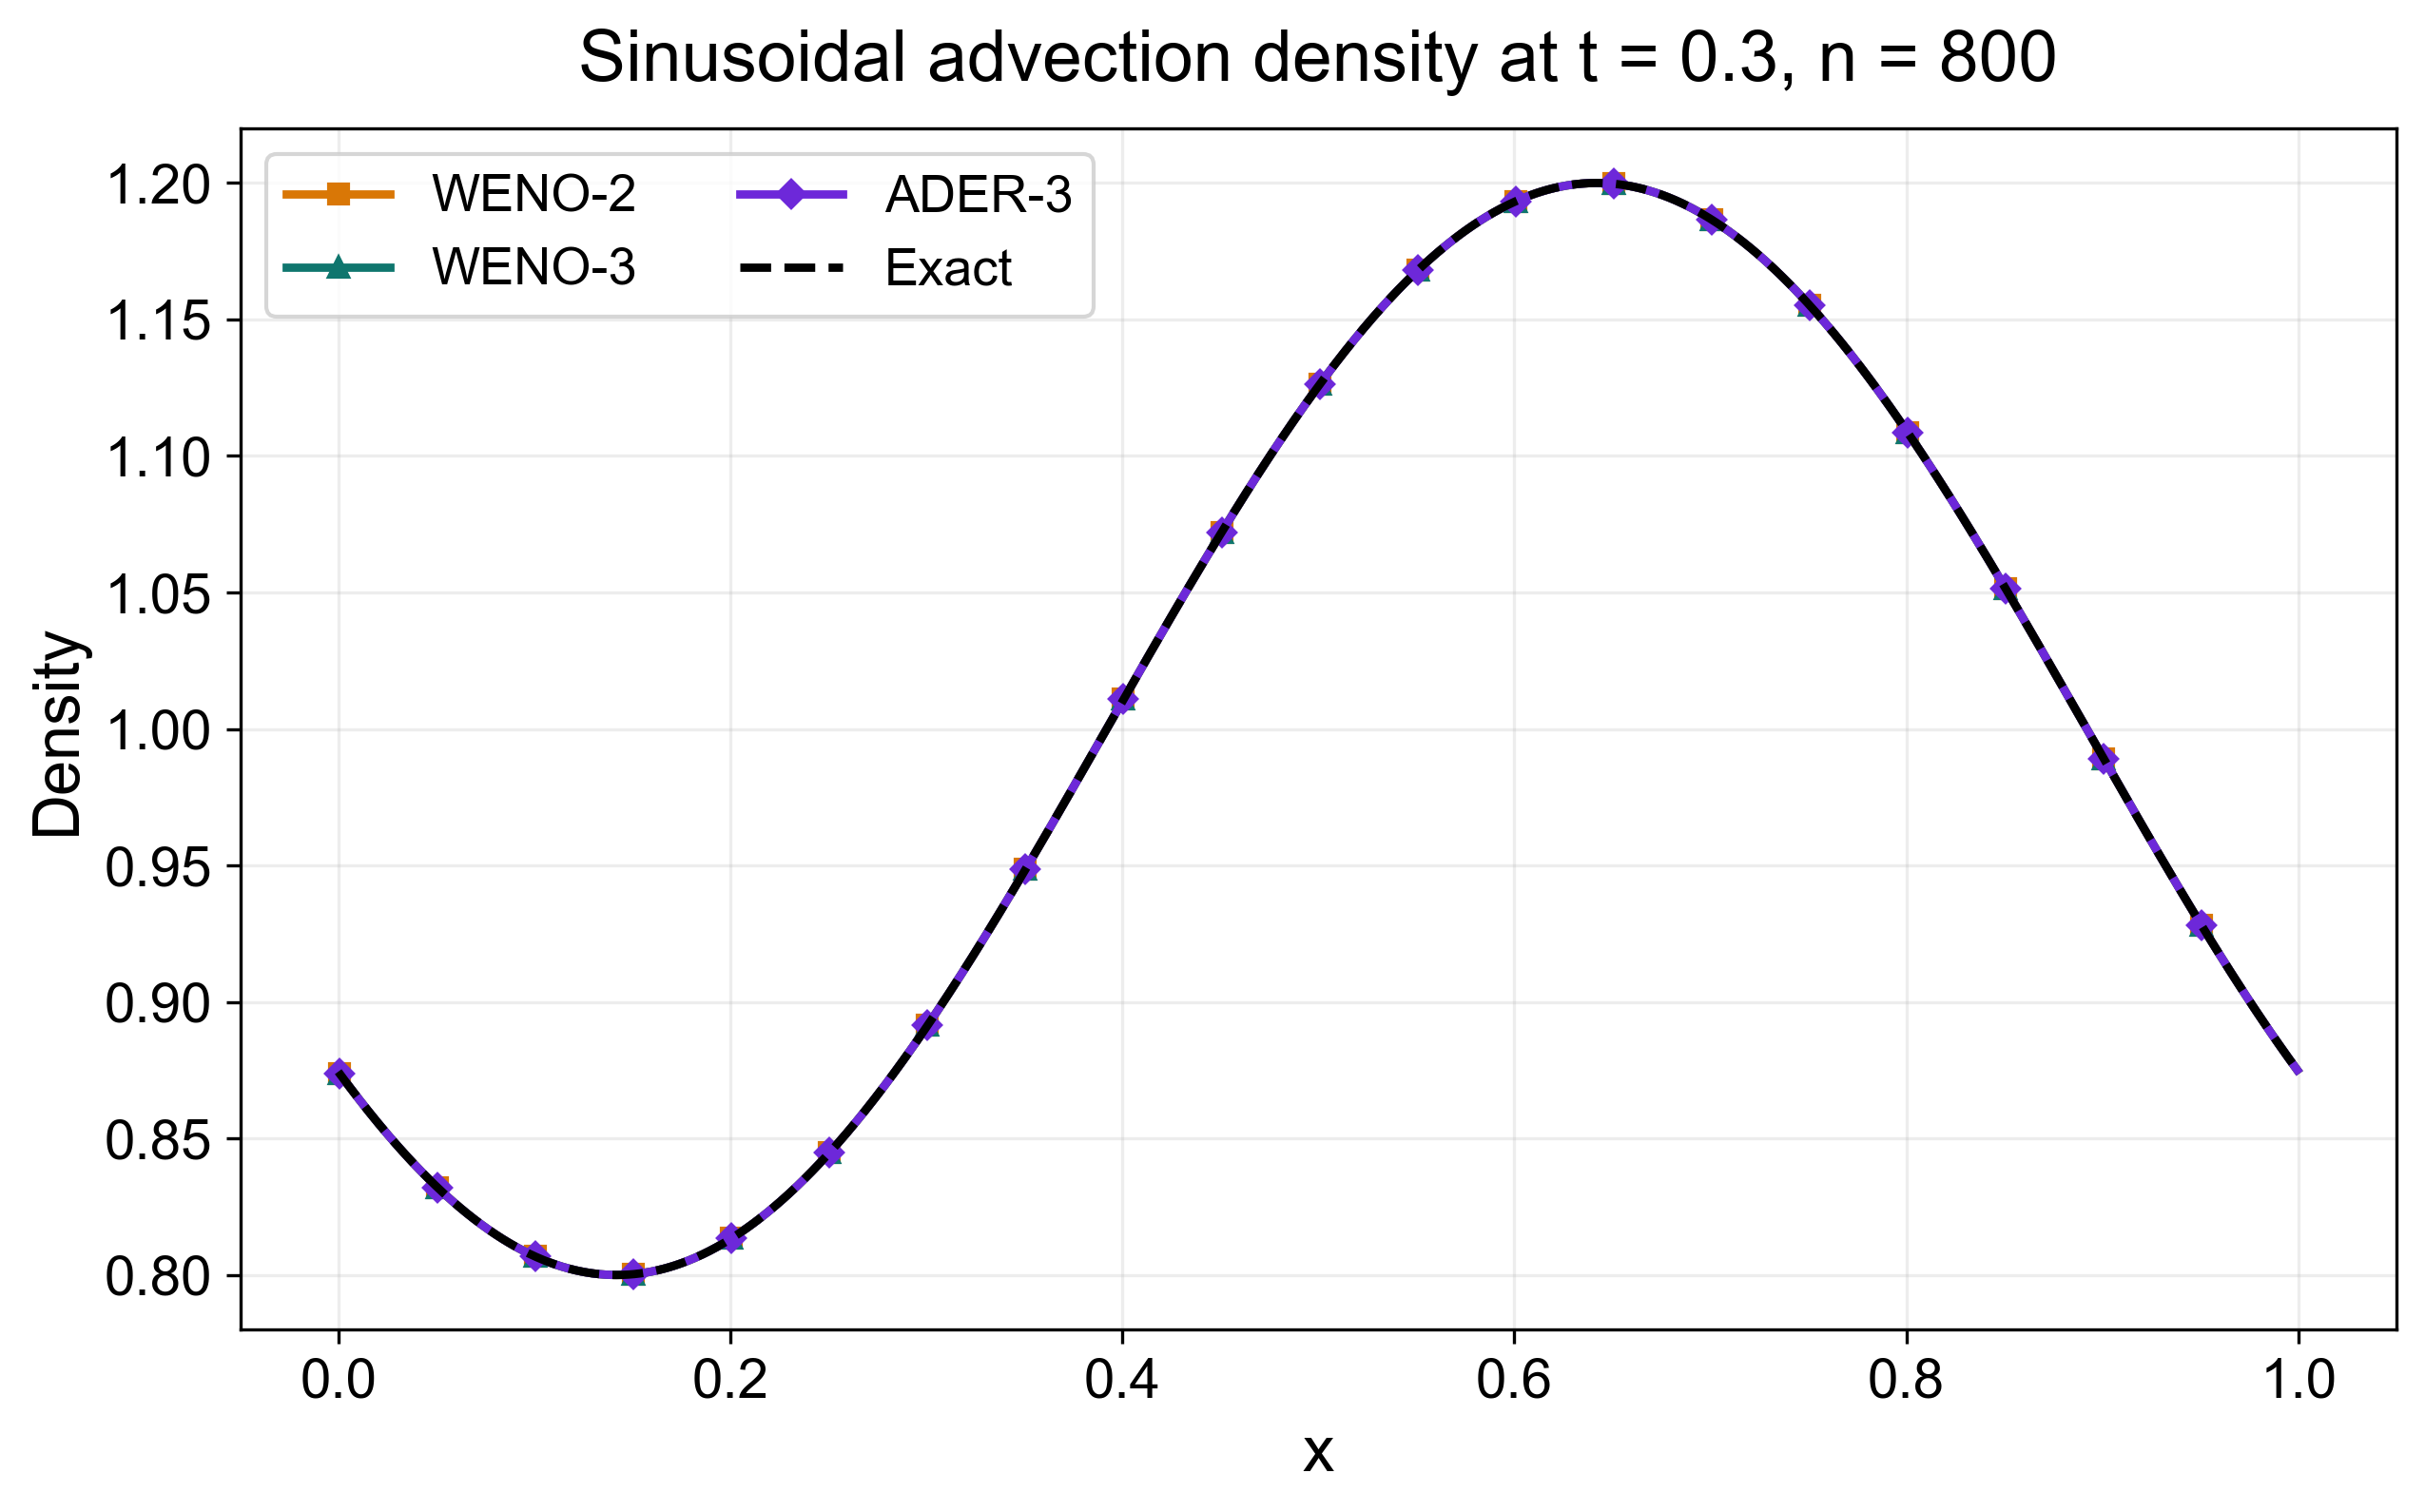
\includegraphics[width=\linewidth]{smooth_advection_hllc_n800.png}
\caption{Sinusoidal advection.}
\end{subfigure}\hfill
\begin{subfigure}[t]{0.49\textwidth}
\centering
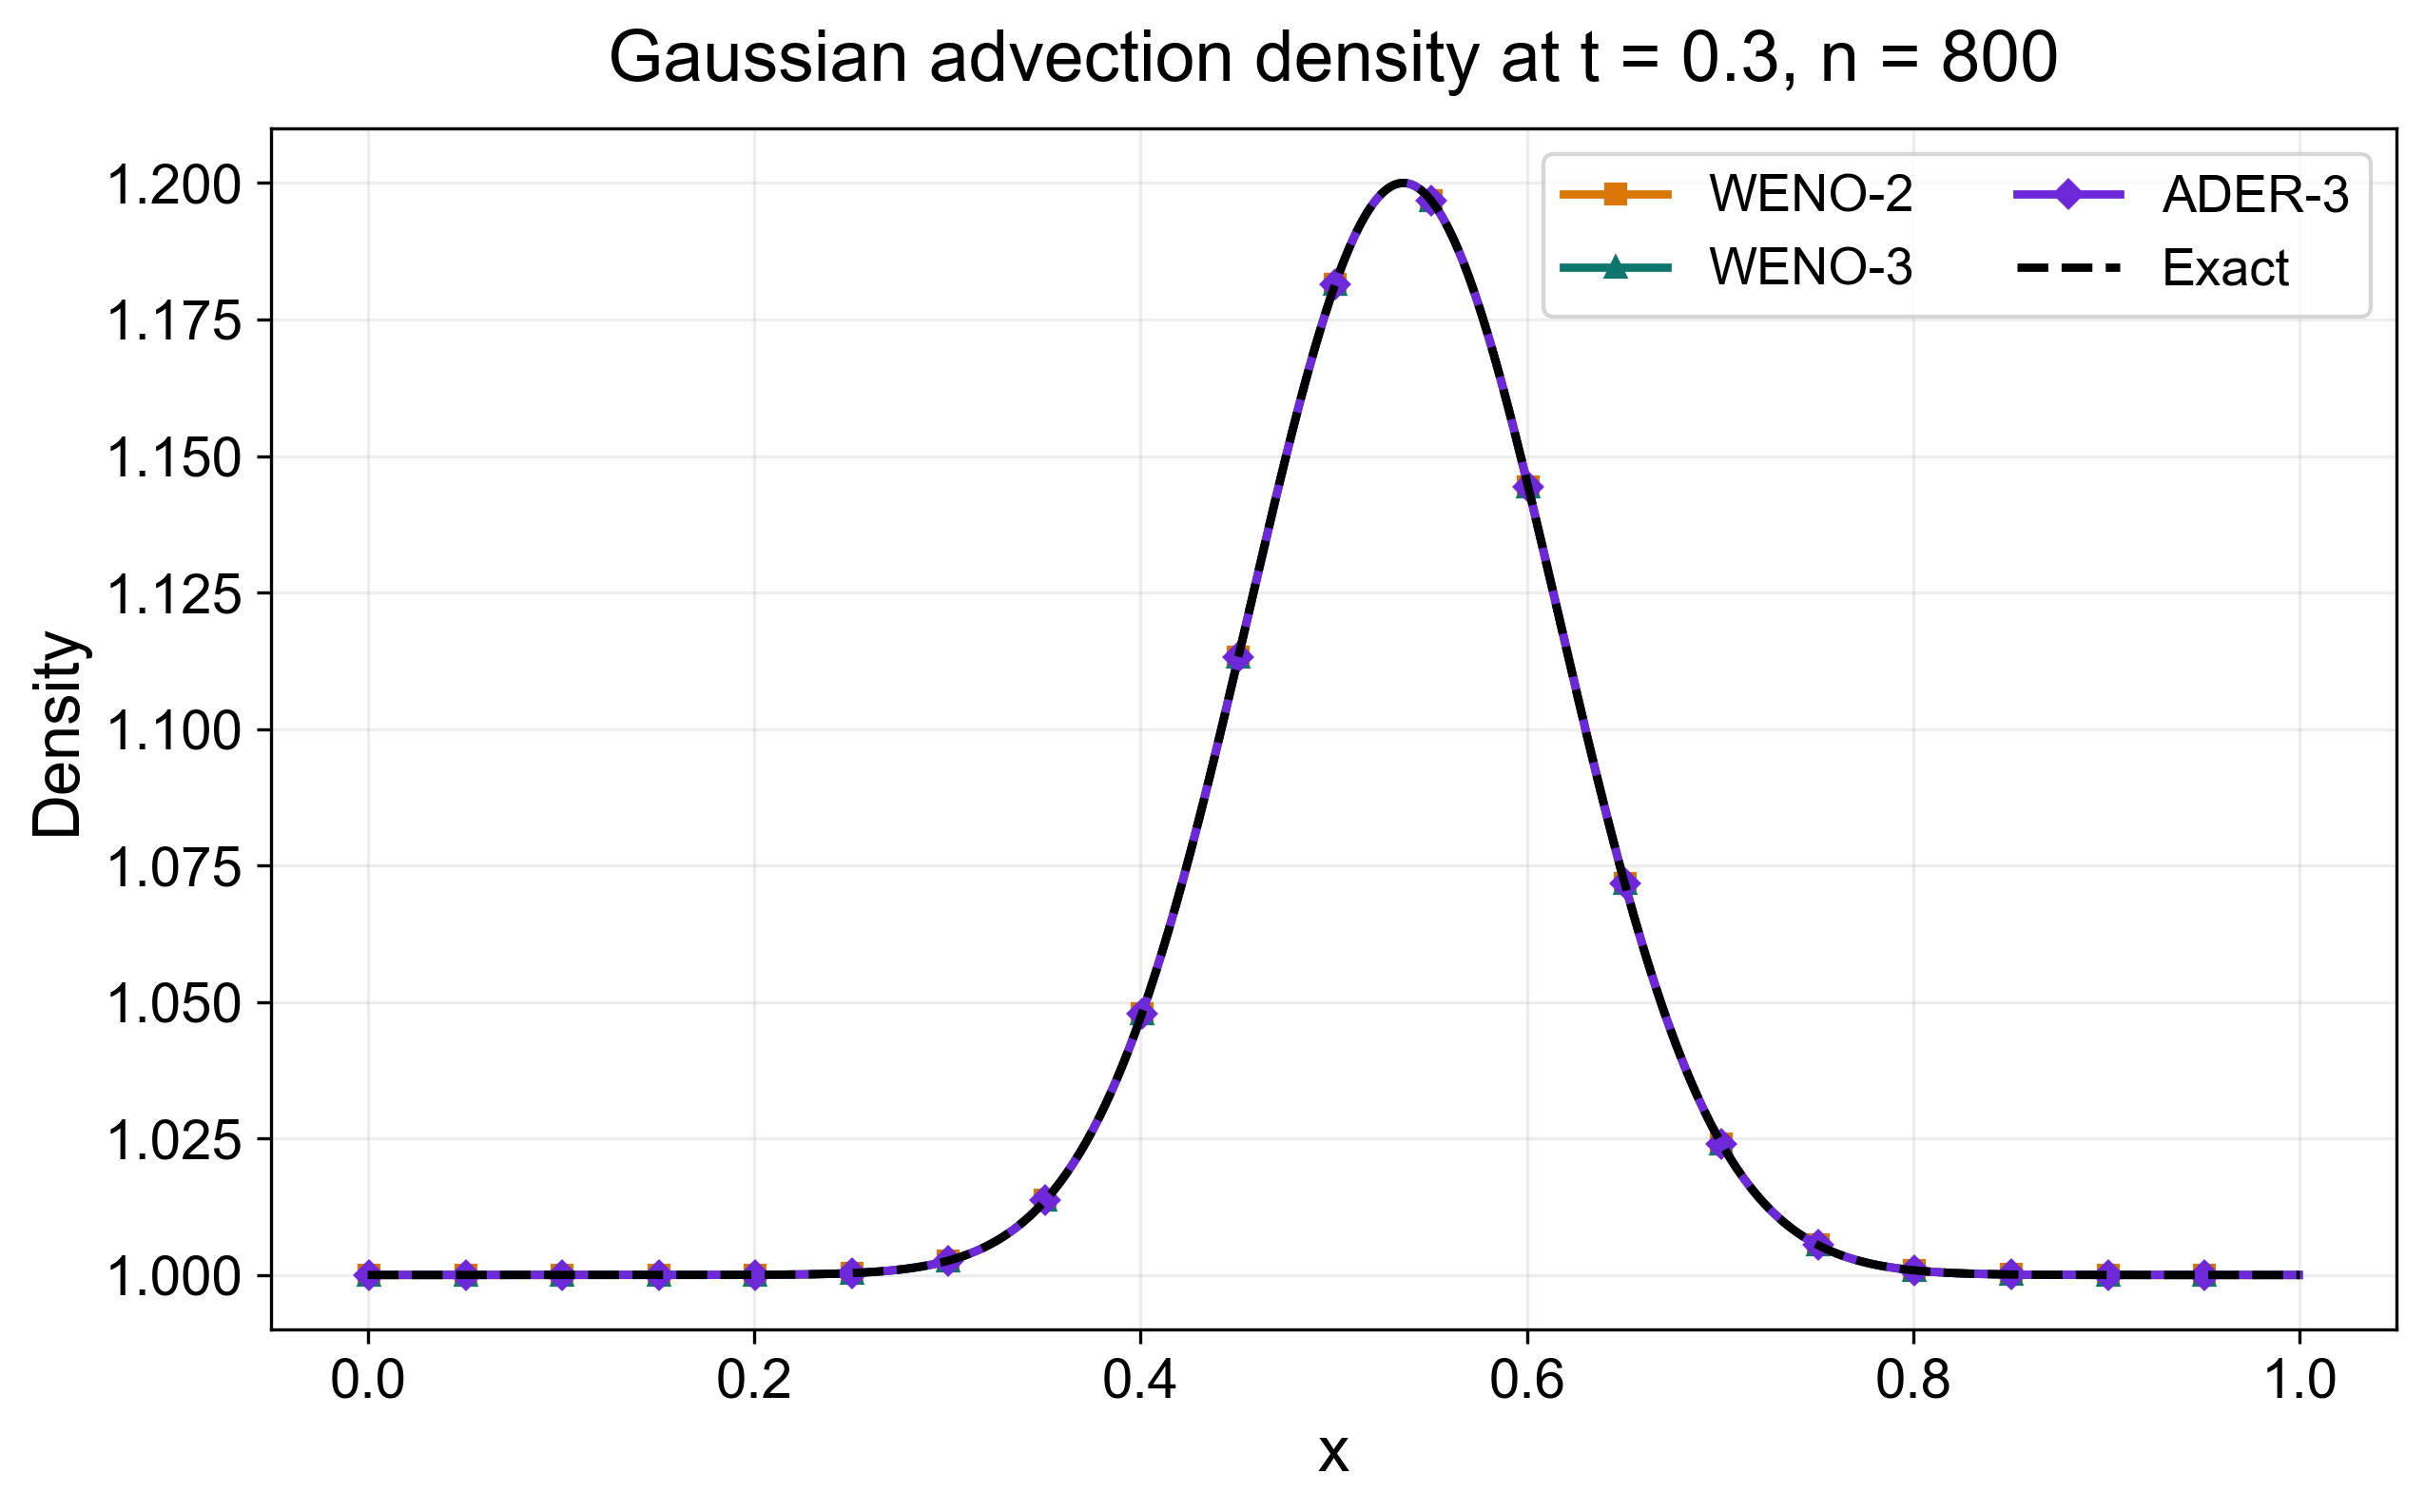
\includegraphics[width=\linewidth]{gaussian_advection_1d_hllc_n800.png}
\caption{Gaussian advection.}
\end{subfigure}
\caption{One-dimensional continuous HLLC validation at \(t=0.3\) and \(n=800\).
The dashed curves are exact cell-average solutions. Numerical markers are thinned for
readability.}
\label{fig:continuous-1d-fields}
\end{figure}

The numerical curves are visually coincident with the exact profiles: the sinusoid has
no resolved phase displacement and the Gaussian peak has no visible shift or flattening.
The corresponding convergence study in Chapter~\ref{chap:validation}, specifically
Figure~\ref{fig:conv1d} and Tables~\ref{tab:conv1d-smooth}--\ref{tab:conv1d-gaussian},
quantifies the \(L_1(\rho)\) errors that are too small to distinguish in
Figure~\ref{fig:continuous-1d-fields}. It shows WENO-2 approaching second order and
WENO-3 and ADER-3 approaching third order through \(n=1600\).

\subsection*{Discontinuous reference}

The Sod shock tube complements that continuous evidence with an exact discontinuous
reference. Its Riemann solution contains a rarefaction, contact discontinuity and shock,
so it tests whether the methods preserve the correct wave ordering and locations.
Figure~\ref{fig:sod-hllc} compares all three HLLC methods with that reference at
\(n=800\).

\begin{figure}[!htbp]
\centering
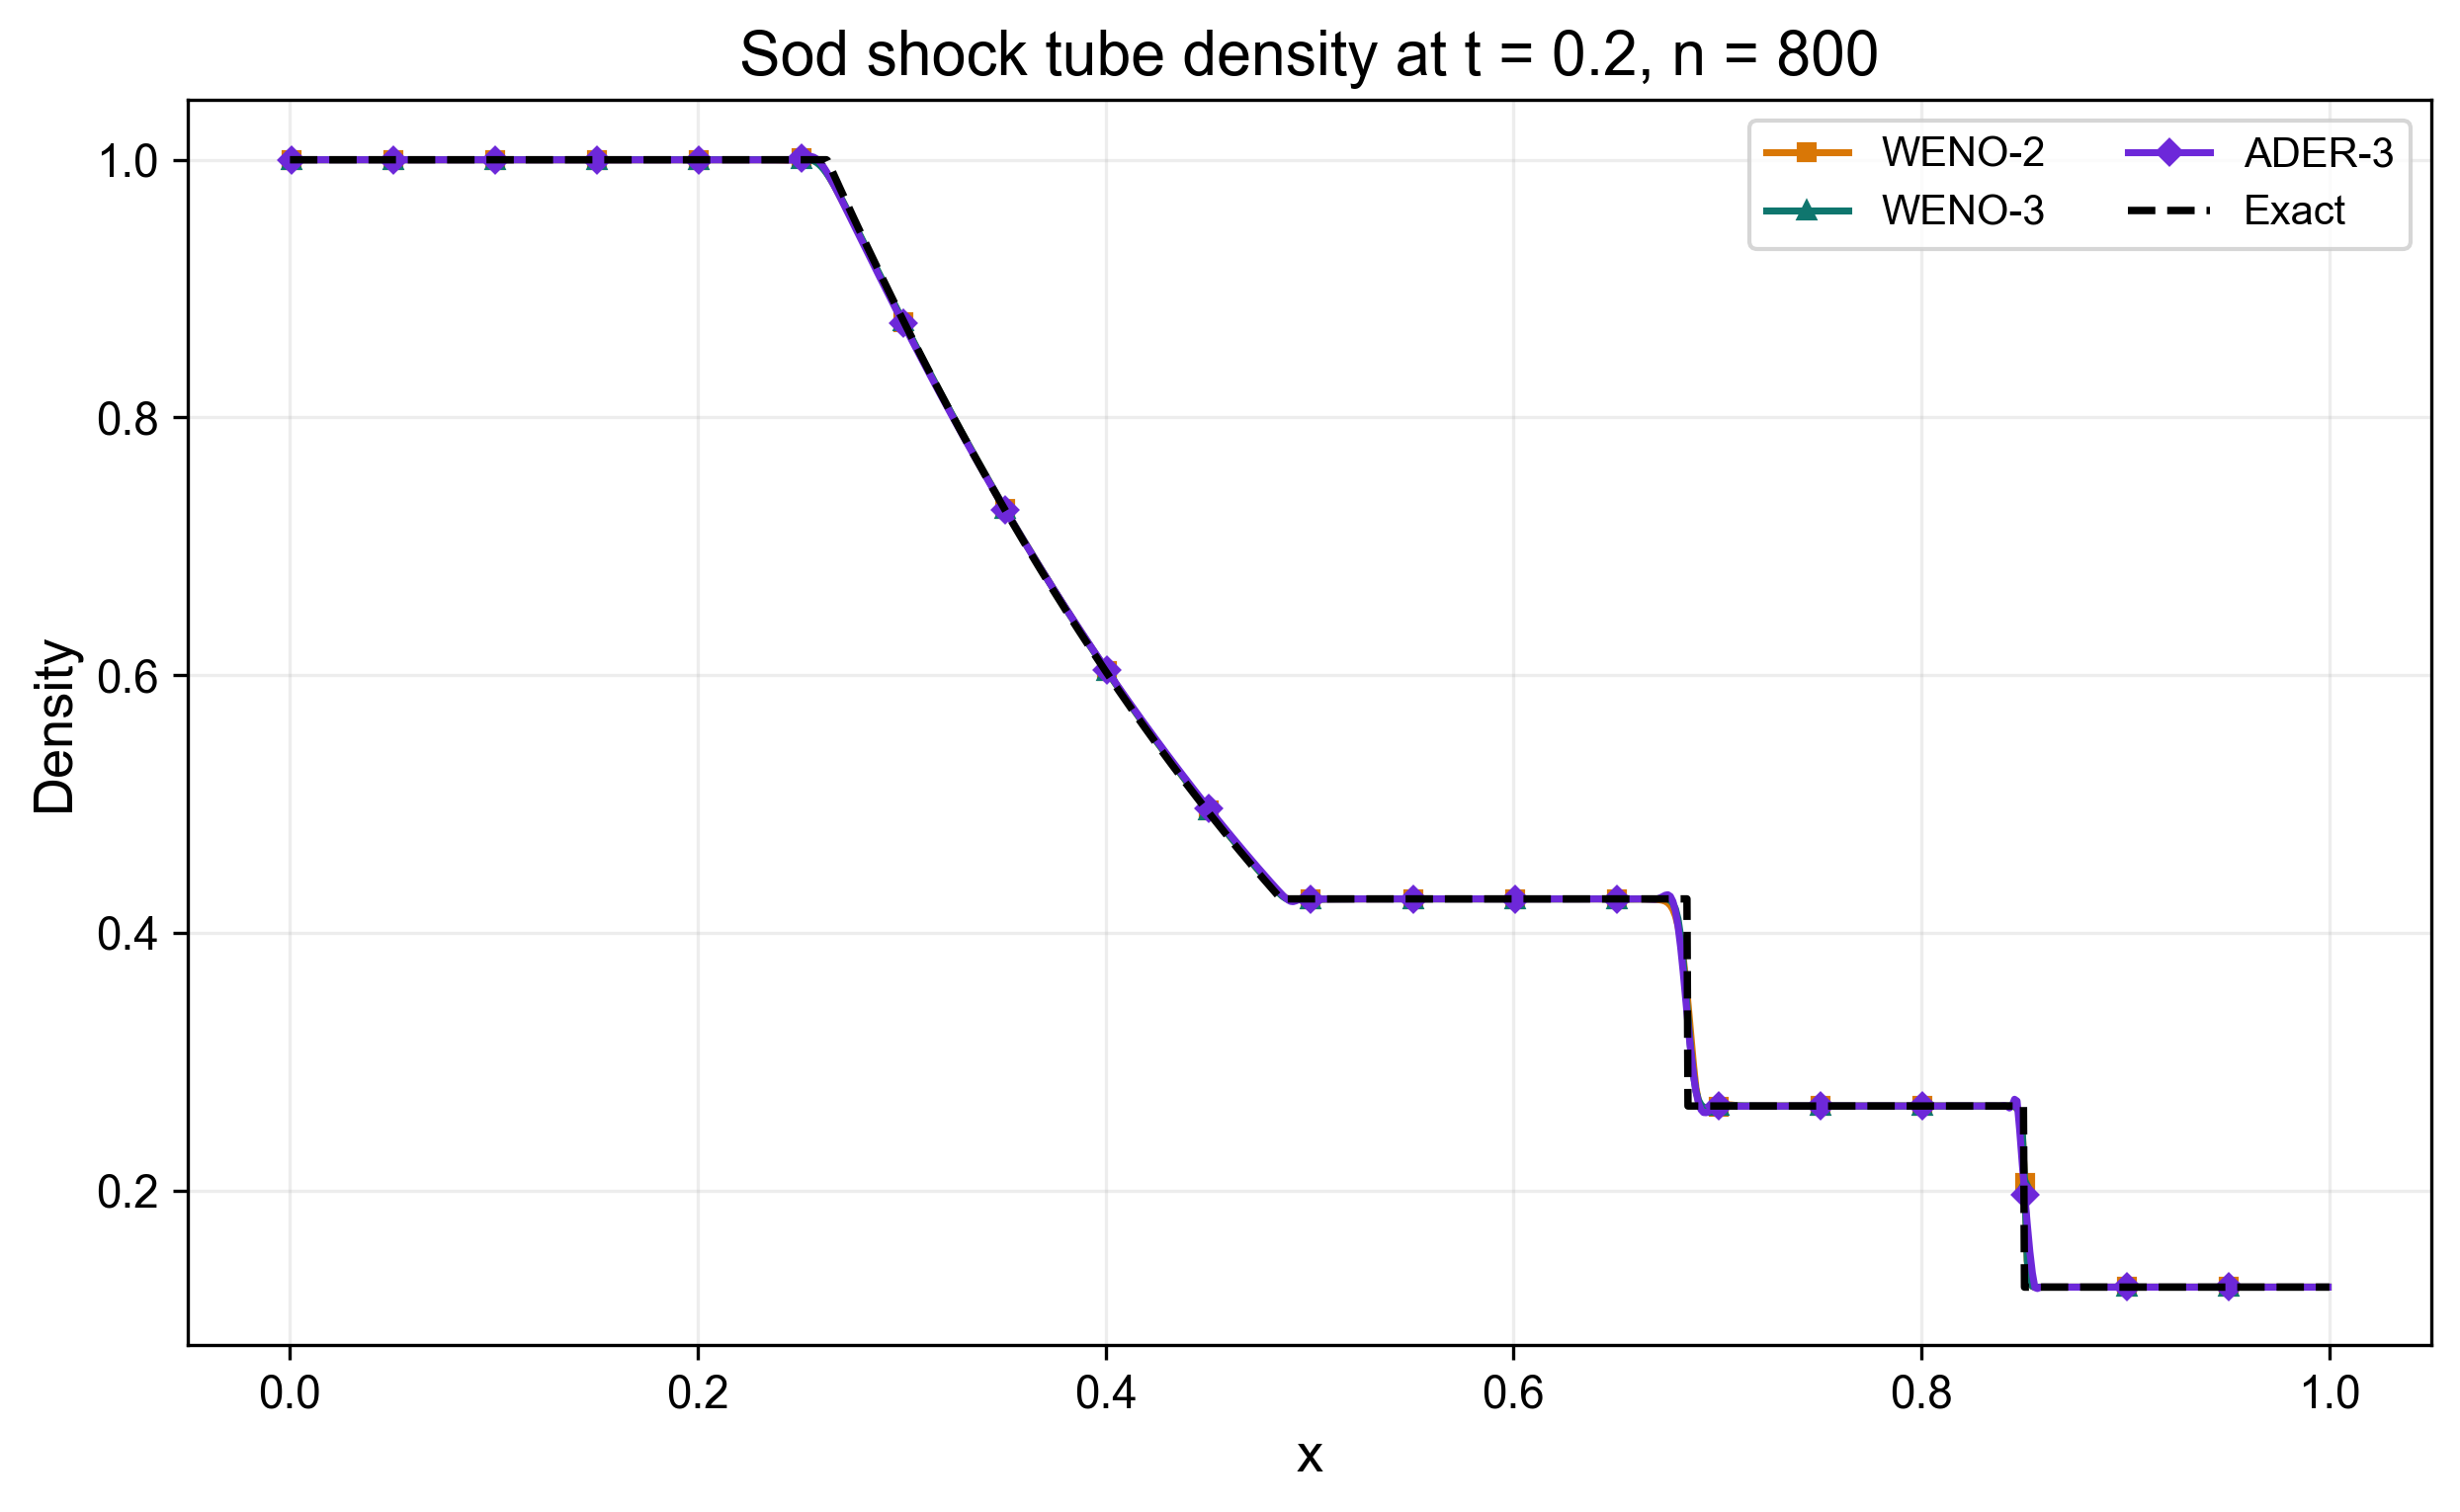
\includegraphics[width=0.91\textwidth]{sod_hllc_n800.png}
\caption{Sod shock-tube density at \(t=0.2\) and \(n=800\). The dashed curve is the exact Riemann solution. Markers are thinned for readability.}
\label{fig:sod-hllc}
\end{figure}

All methods reproduce the rarefaction endpoints, contact and shock locations without a
visible phase error. Their finite thickness is expected for a non-oscillatory finite-volume
solution. Method separation is confined to a few cells around the contact and shock:
WENO-2 gives the broadest transition, while WENO-3 and ADER-3 follow the exact plateaux
more tightly without visible ringing. The recovered contact also verifies the middle-wave
star region in Equation~\eqref{eq:hllcflux} before the analysis moves to interacting
two-dimensional waves.

\section{CFL sensitivity in discontinuous ADER-3}
\label{sec:cfl-study}

The discontinuous ADER-3 calculation required a separate CFL study before the backend comparison could be fixed. This was not a search for a CFL that made one backend appear faster. For every trial, serial and CUDA used the same grid, final time, boundary conditions, HLLC flux and CFL number. The measured quantity was the maximum absolute difference between their exported fields. The two discontinuous problems responded differently because small changes in the accepted time-step sequence can move reconstructed states across an admissibility or troubled-interface threshold.

\begin{table}[H]
\centering
\small
\renewcommand{\arraystretch}{1.18}
\begin{tabular}{@{}ccc>{\raggedright\arraybackslash}p{0.43\textwidth}@{}}
\toprule
CFL & Quadrant Riemann & Shock--bubble & Interpretation \\
\midrule
0.10 & $1.60\times10^{-12}$ & $3.96\times10^{-4}$ & Quadrant stable, shock--bubble branch-sensitive \\
0.12 & $3.36\times10^{-3}$ & $<6\times10^{-8}$ & Shock--bubble stable, quadrant branch-sensitive \\
0.13 & $5.03\times10^{-12}$ & $1.58\times10^{-2}$ & Quadrant stable, shock--bubble mismatch \\
0.14 & $3.68\times10^{-12}$ & $2.02\times10^{-7}$ & Best common compromise \\
0.15 & $4.93\times10^{-12}$ & $\mathcal{O}(10^{-3})$ & Shock--bubble mismatch returns \\
\bottomrule
\end{tabular}
\caption{ADER-3 CFL study used to select the common discontinuous-test value. Entries are the largest absolute CUDA--serial field differences.}
\label{tab:ader3-cfl-study}
\end{table}

The response is non-monotone: reducing CFL does not necessarily reduce the backend difference. A different CFL changes the sequence of accepted time steps, reconstructed interface states and the locations at which the positivity/fallback logic is activated. Values close to a branch threshold can therefore send serial and CUDA through different locally admissible paths even though both calculations remain finite. CFL 0.14 is the only tested common value that keeps the quadrant result near roundoff and the shock--bubble discrepancy below $3\times10^{-7}$. It is consequently used for ADER-3 in all discontinuous backend comparisons. WENO-2 and WENO-3 use CFL 0.20, for which no comparable branch sensitivity was observed.

\FloatBarrier
\section{Two-dimensional physical fields and backend differences}
\label{sec:resolved-fields}

The \(600\times600\) fields below provide the physical reference at a resolution high
enough to expose smooth peaks, shocks and contacts clearly. Backend differences are
measured separately at \(100\times100\), where complete serial, OpenMP and CUDA fields
are compared cell by cell. The two resolutions serve different purposes: the former shows
what was resolved, whereas the latter isolates implementation-dependent differences at
manageable storage cost.

\subsection*{Gaussian advection}

\begin{figure}[!htbp]
\centering
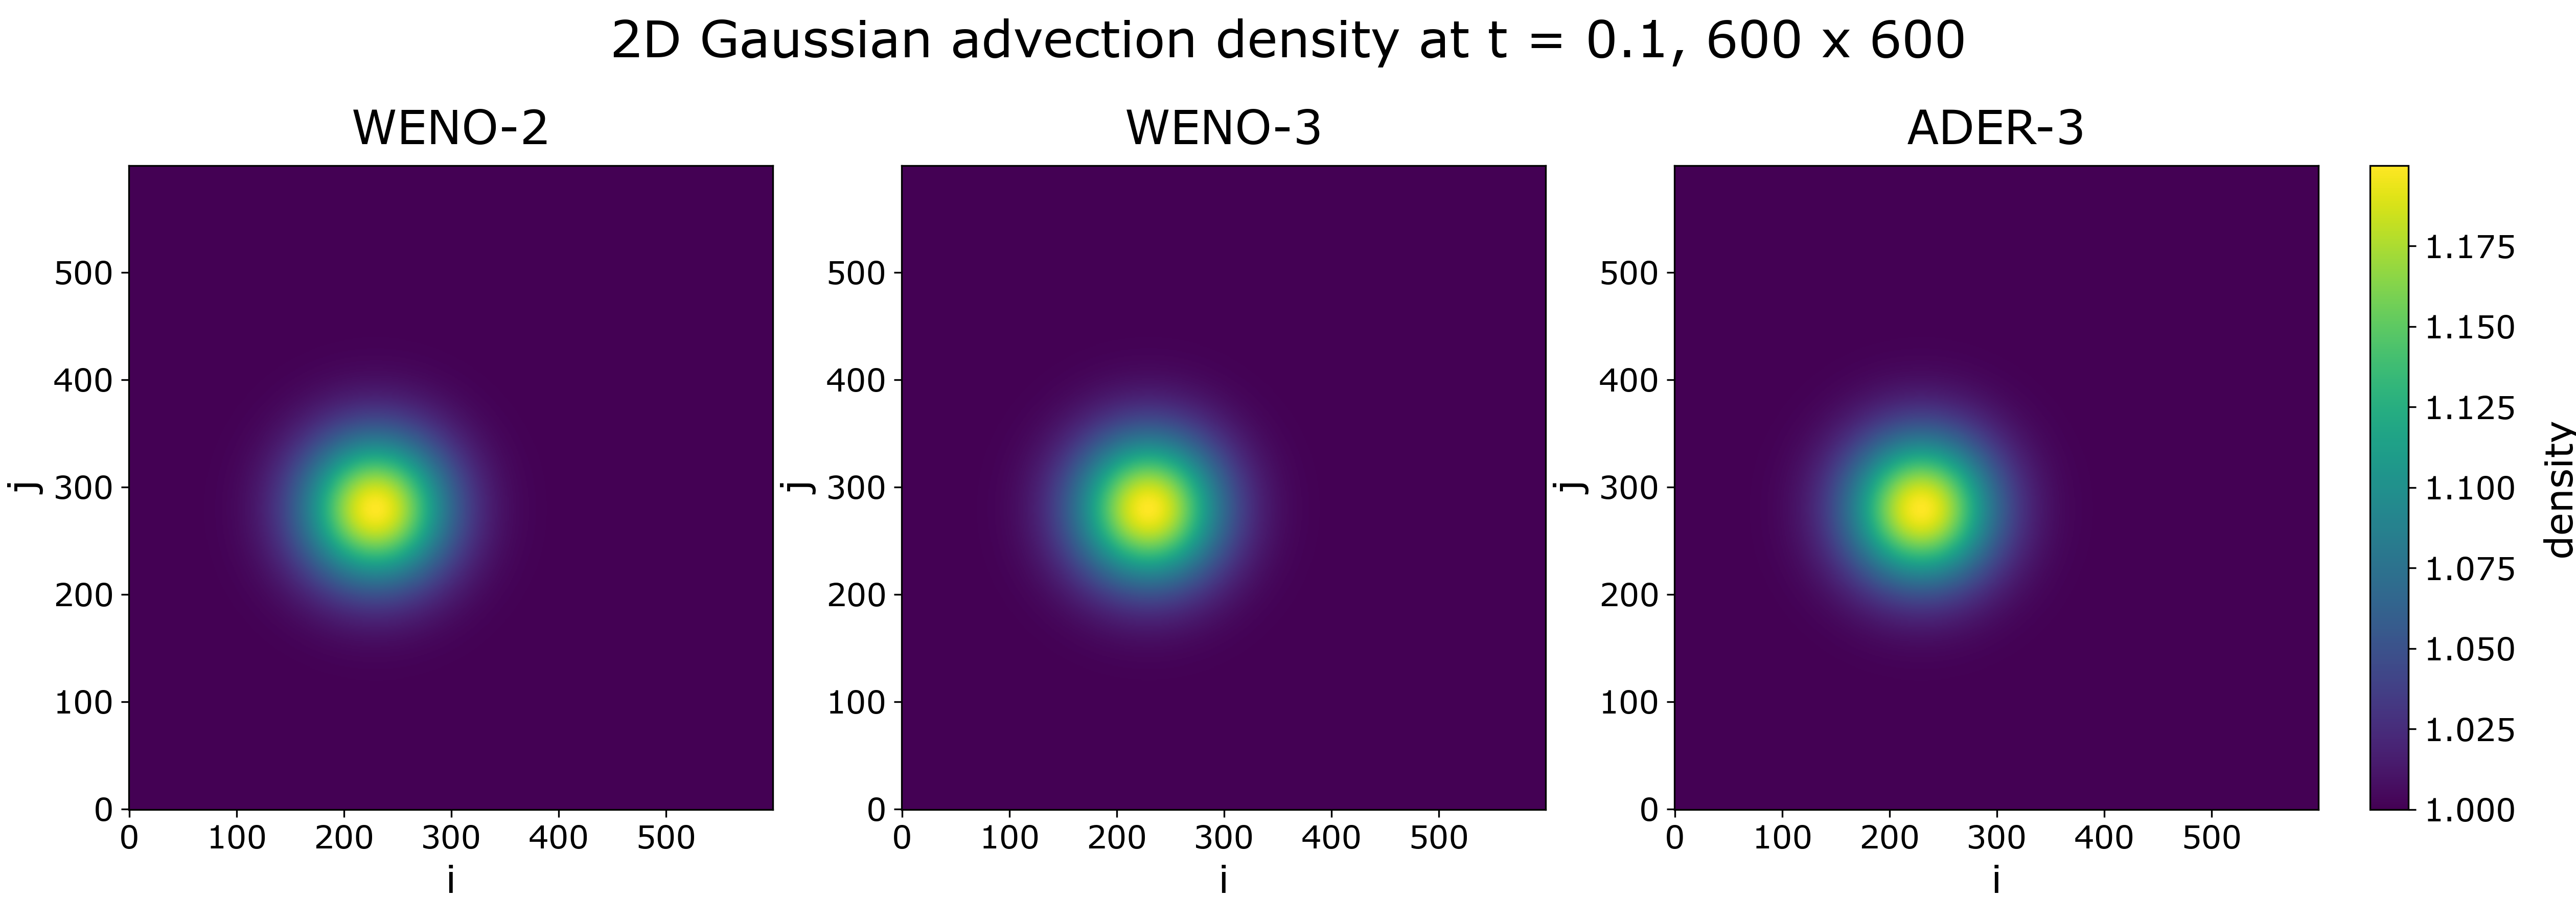
\includegraphics[width=0.98\textwidth]{gaussian_advection_hllc_n600.png}
\caption{HLLC density fields for two-dimensional Gaussian advection at \(t=0.1\) and
\(600\times600\). All methods transport the pulse to the same location and preserve a
smooth, symmetric field. WENO-3 and ADER-3 retain a slightly more compact peak than
WENO-2.}
\label{fig:gaussian-fields-performance}
\end{figure}

Figure~\ref{fig:gaussian-fields-performance} establishes the smooth-flow reference:
the transported pulse is neither displaced nor visibly distorted. On the common colour
scale, WENO-2 has a slightly broader radial footprint, whereas WENO-3 and ADER-3 retain
a more compact peak. All three remain circular, with no directional wake or grid-aligned
deformation. The backend-difference maps below are therefore interpreted against an
unchanged physical solution.

\begin{figure}[!htbp]
\centering
\begin{subfigure}[t]{0.47\textwidth}
\centering
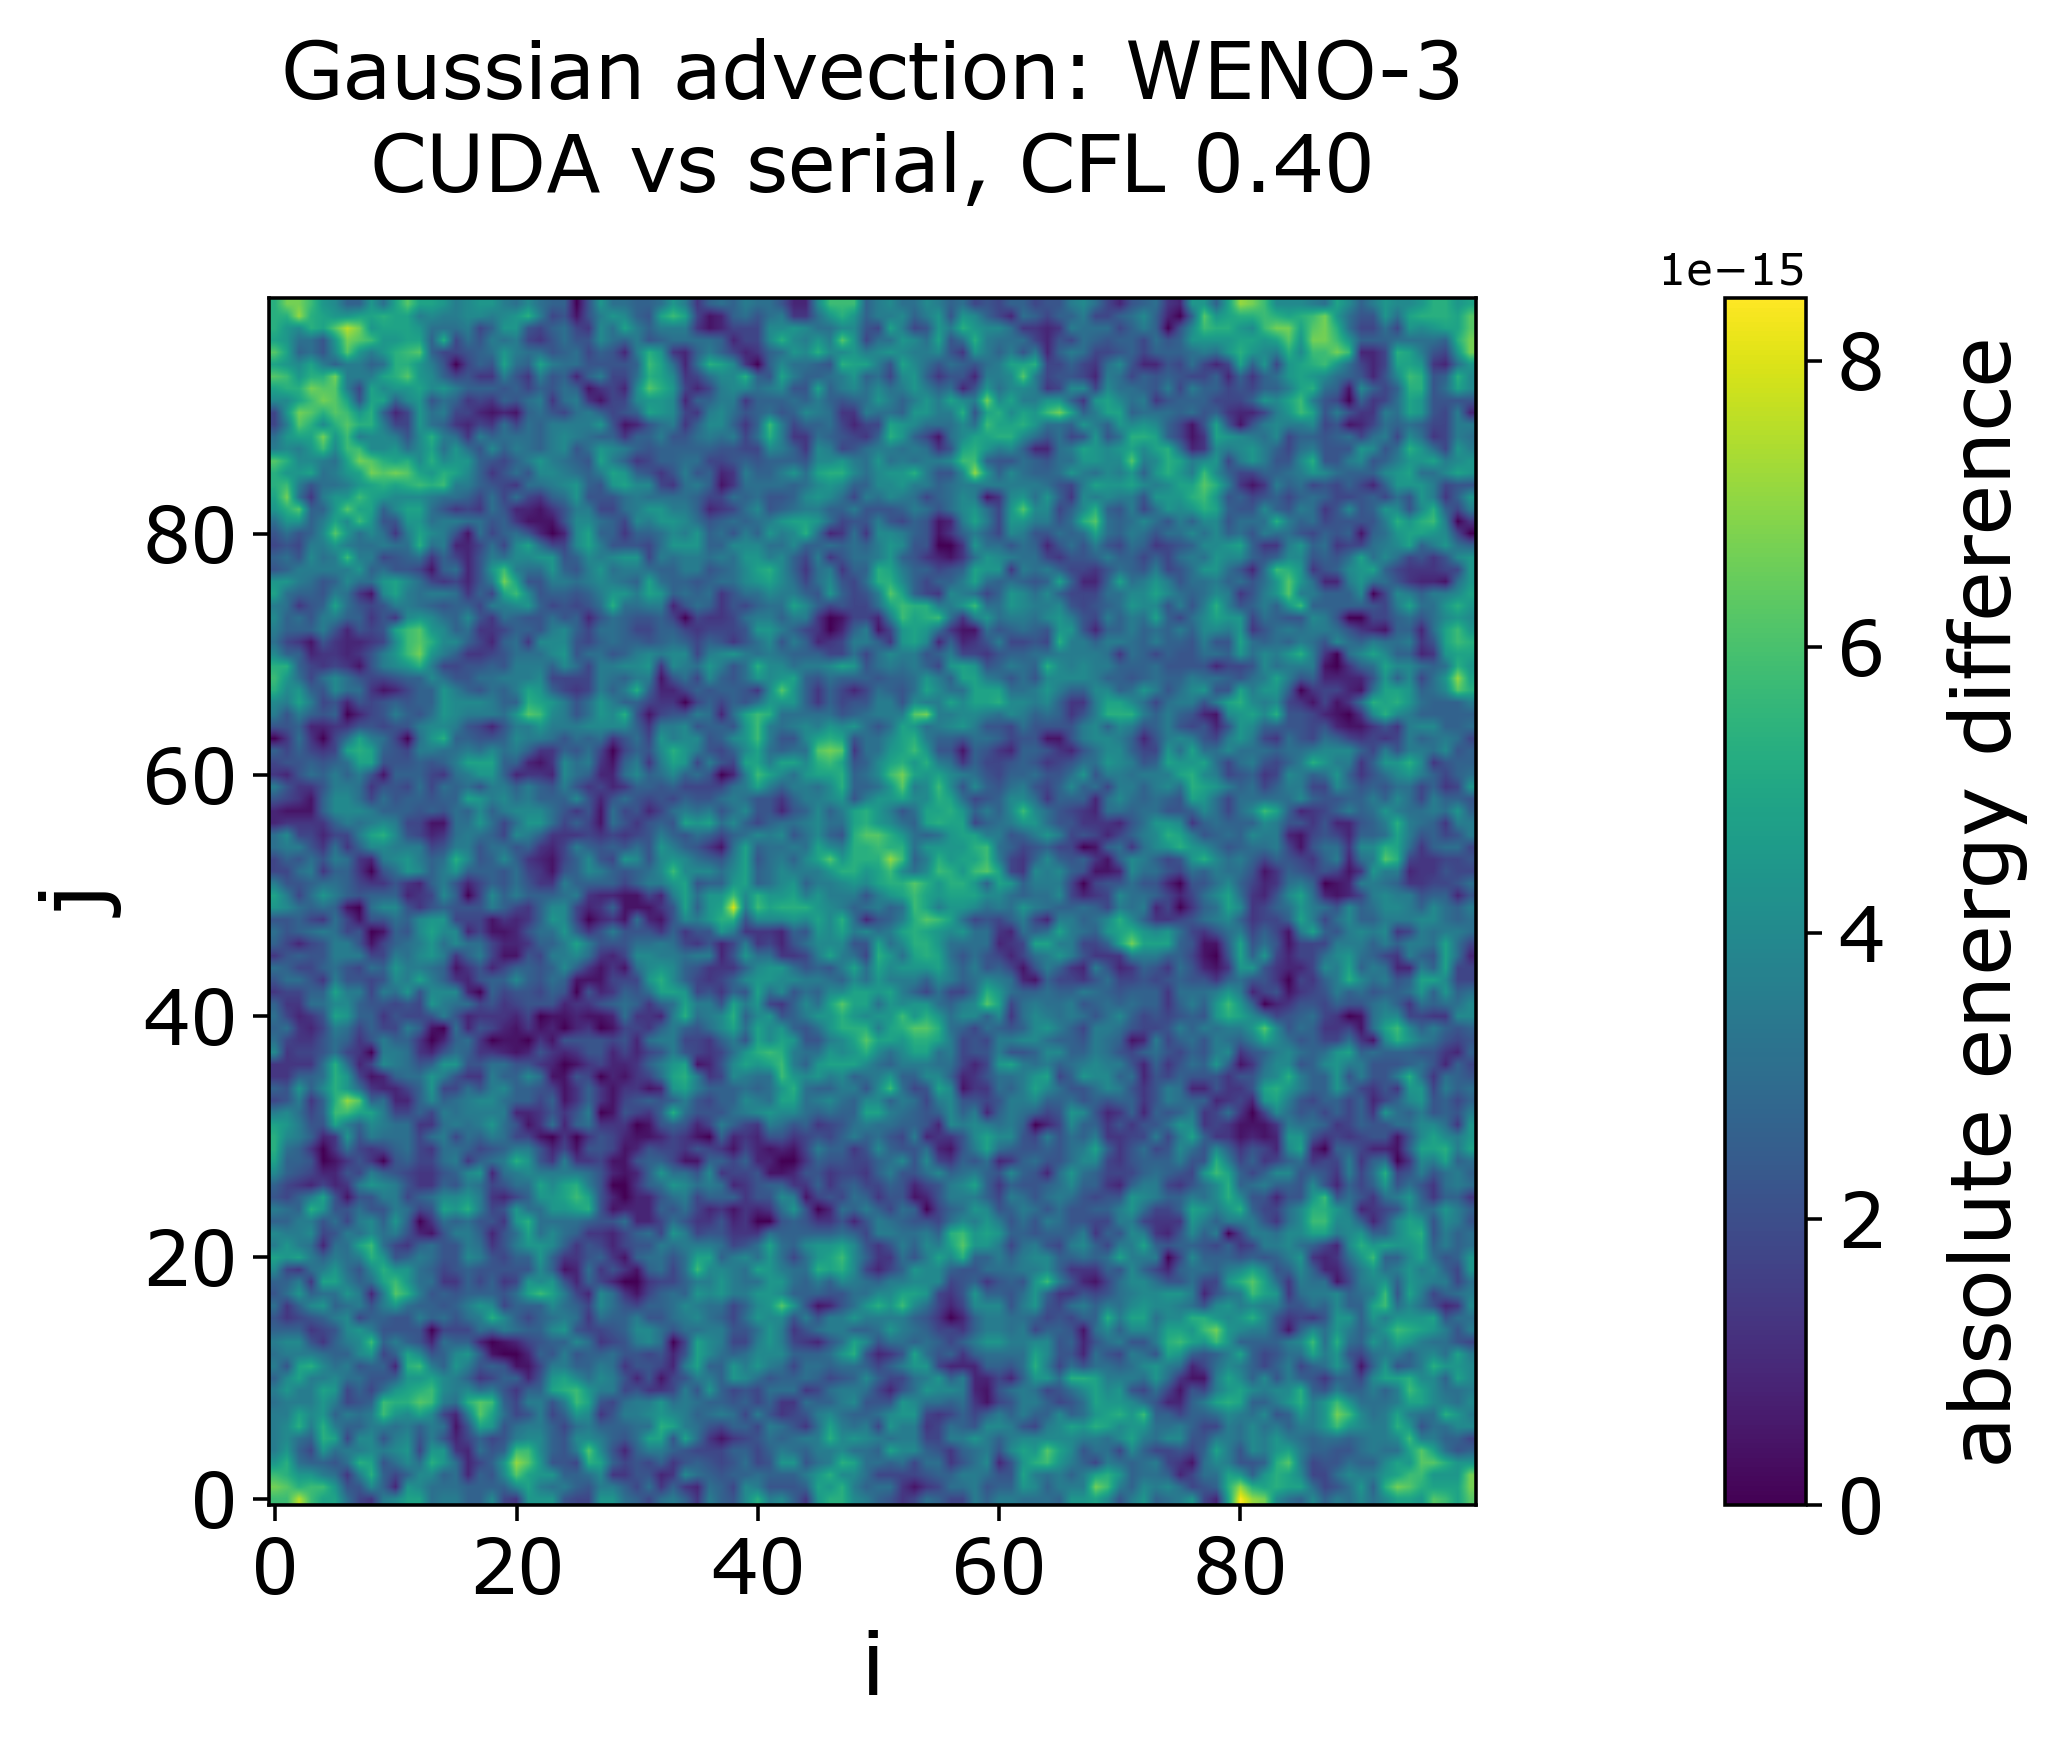
\includegraphics[width=\linewidth]{gaussian_advection_weno3_energy_absdiff.png}
\caption{WENO-3: $\max|\Delta E|=8.438\times10^{-15}$.}
\end{subfigure}\hfill
\begin{subfigure}[t]{0.47\textwidth}
\centering
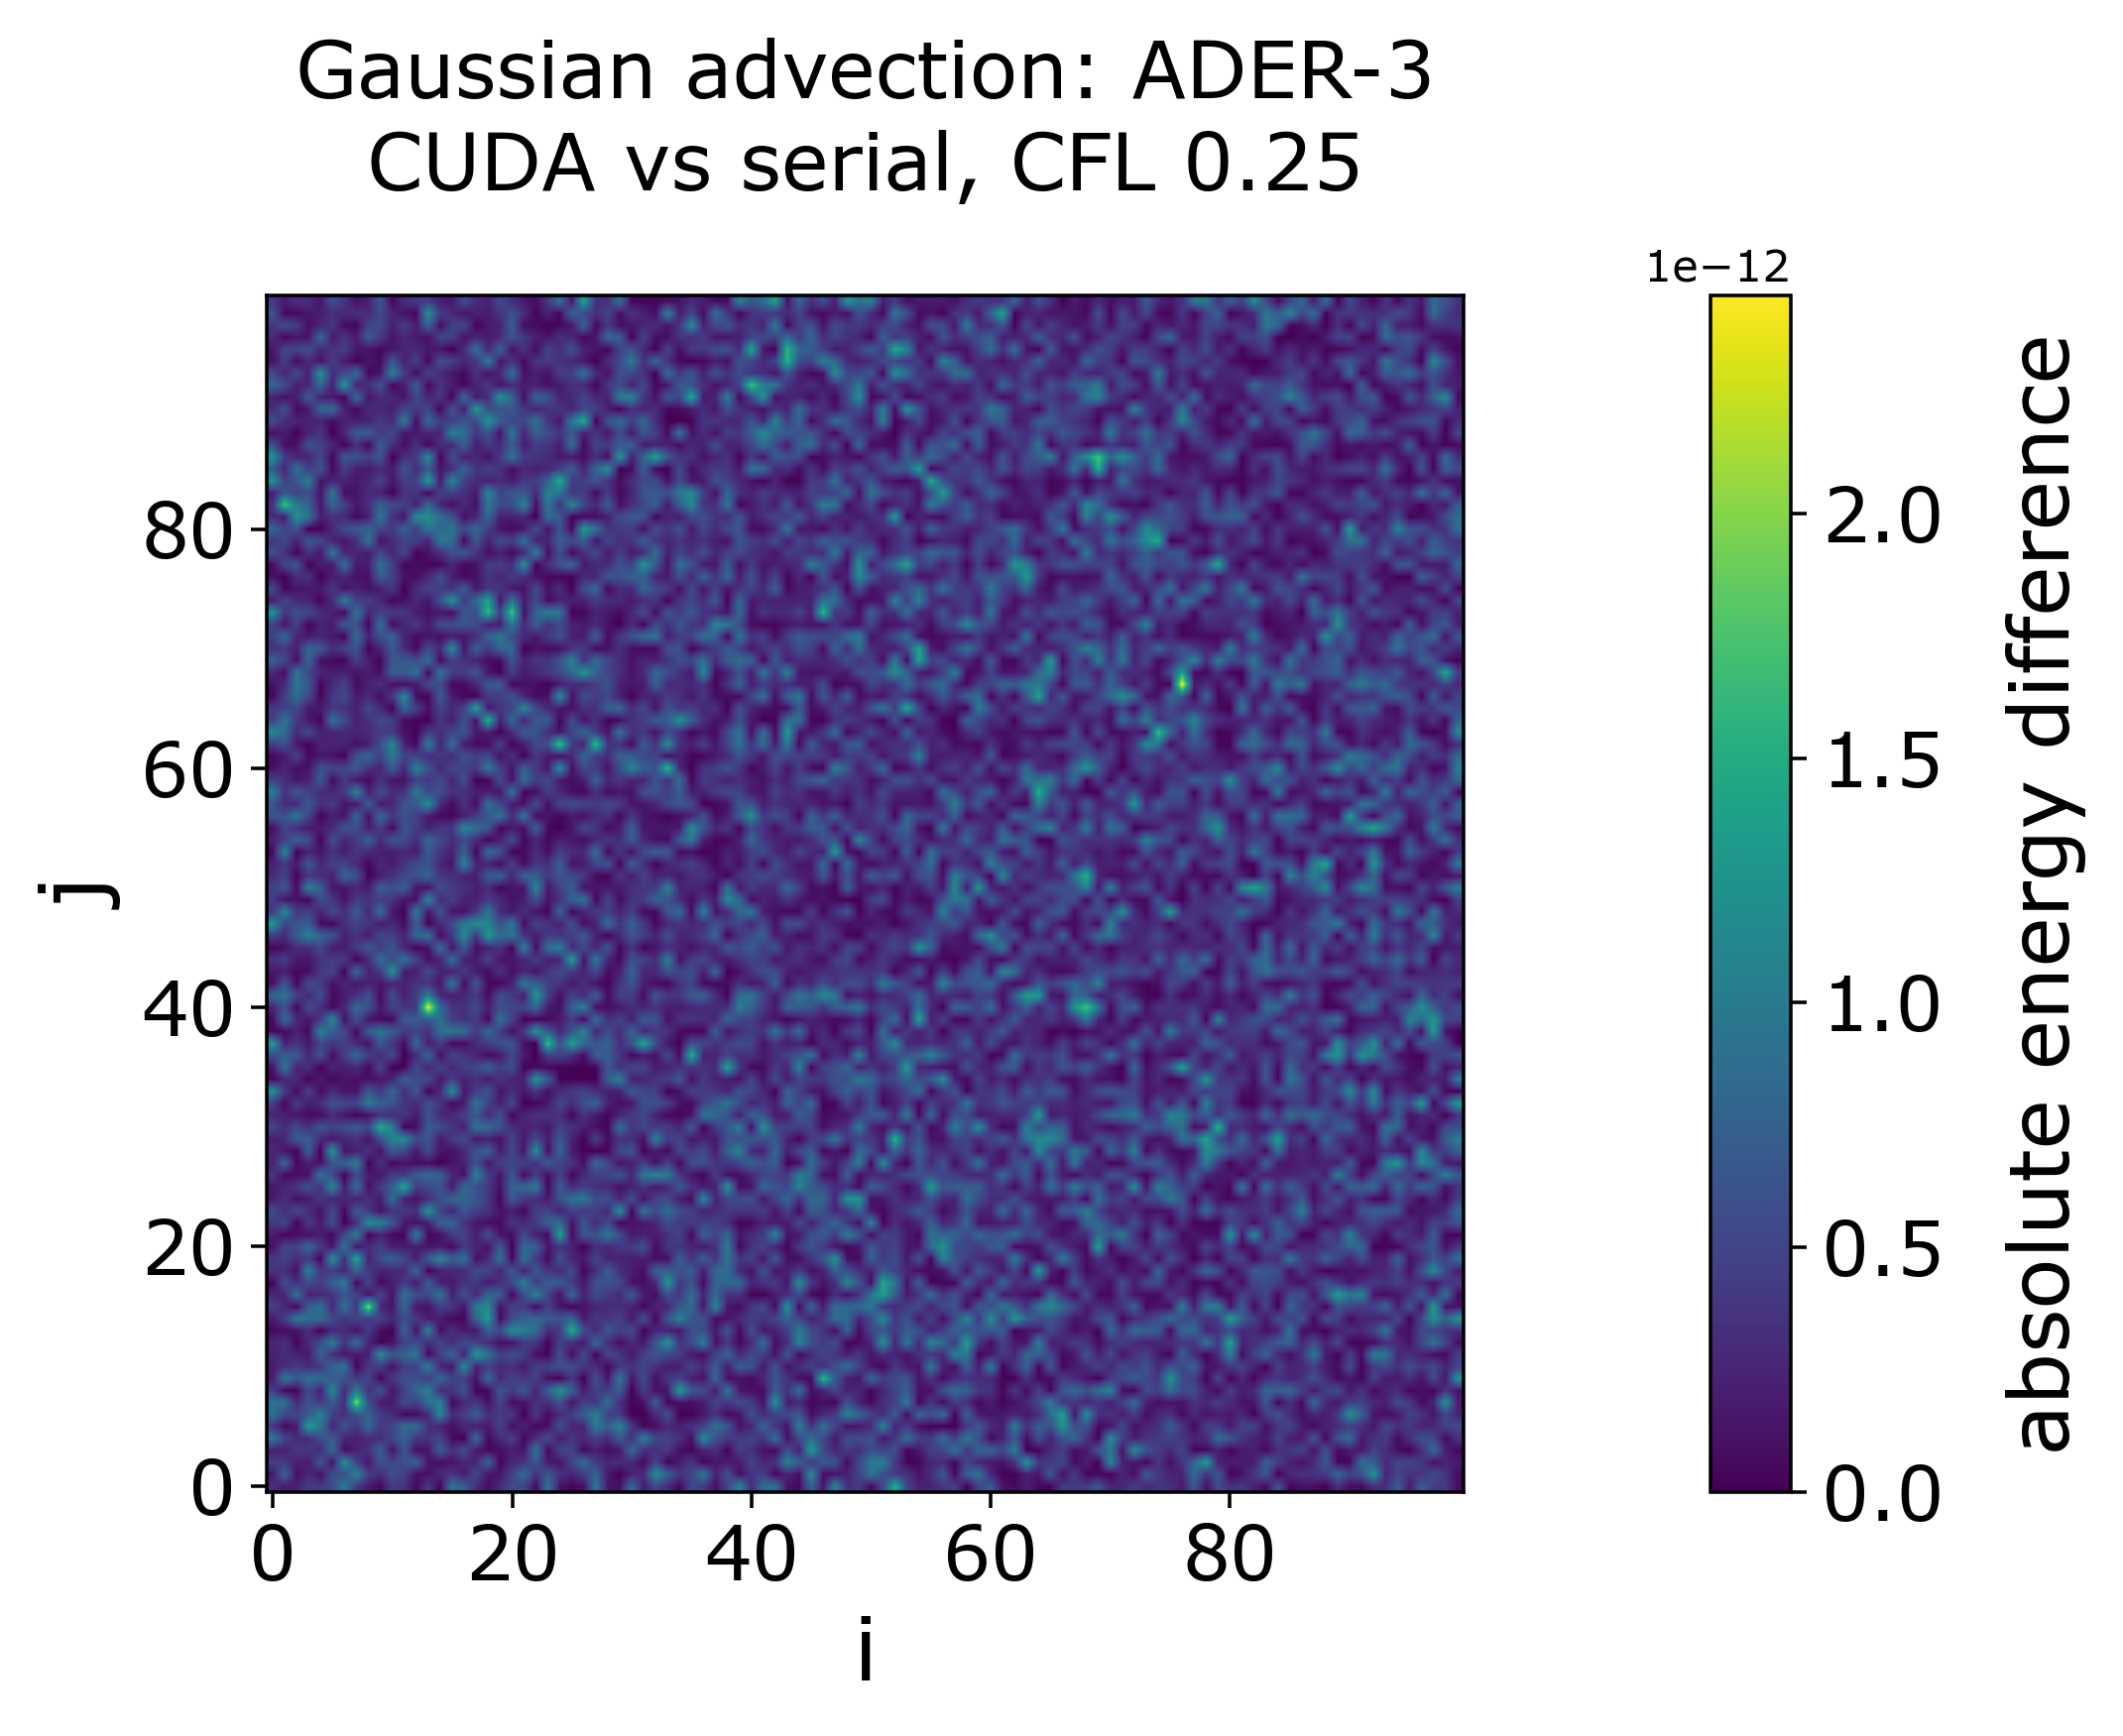
\includegraphics[width=\linewidth]{gaussian_advection_ader3_energy_absdiff.png}
\caption{ADER-3: $\max|\Delta E|=2.445\times10^{-12}$.}
\end{subfigure}
\caption{Absolute CUDA--serial energy differences for Gaussian advection at $100\times100$. Each panel uses its own colour scale.}
\label{fig:third-order-gaussian-difference}
\end{figure}

The absolute differences are extremely small. WENO-3 remains at
$8.438\times10^{-15}$, while the larger ADER-3 energy difference is
$2.445\times10^{-12}$. Both are many orders of magnitude below the resolved density
variation.

Neither map contains a coherent pulse-aligned pattern. Their domain-wide, fine-scale
distribution is characteristic of accumulated floating-point roundoff rather than a
displaced Gaussian pulse, an incorrect boundary treatment, or a backend-dependent
physical branch.

\FloatBarrier
\subsection*{Quadrant Riemann problem}

The quadrant problem contains several waves that meet near the initial intersection, so
reconstruction, HLLC branch selection and multidimensional coupling act in one compact
region. Figure~\ref{fig:quadrant-evolution-discontinuous} first follows a representative
WENO-3 calculation. The four initial constant states begin to interact by \(t=0.1\).
at \(t=0.2\), the central structure is fully developed while regions beyond the wave
fronts retain their prescribed far-field values.

\begin{figure}[!htbp]
\centering
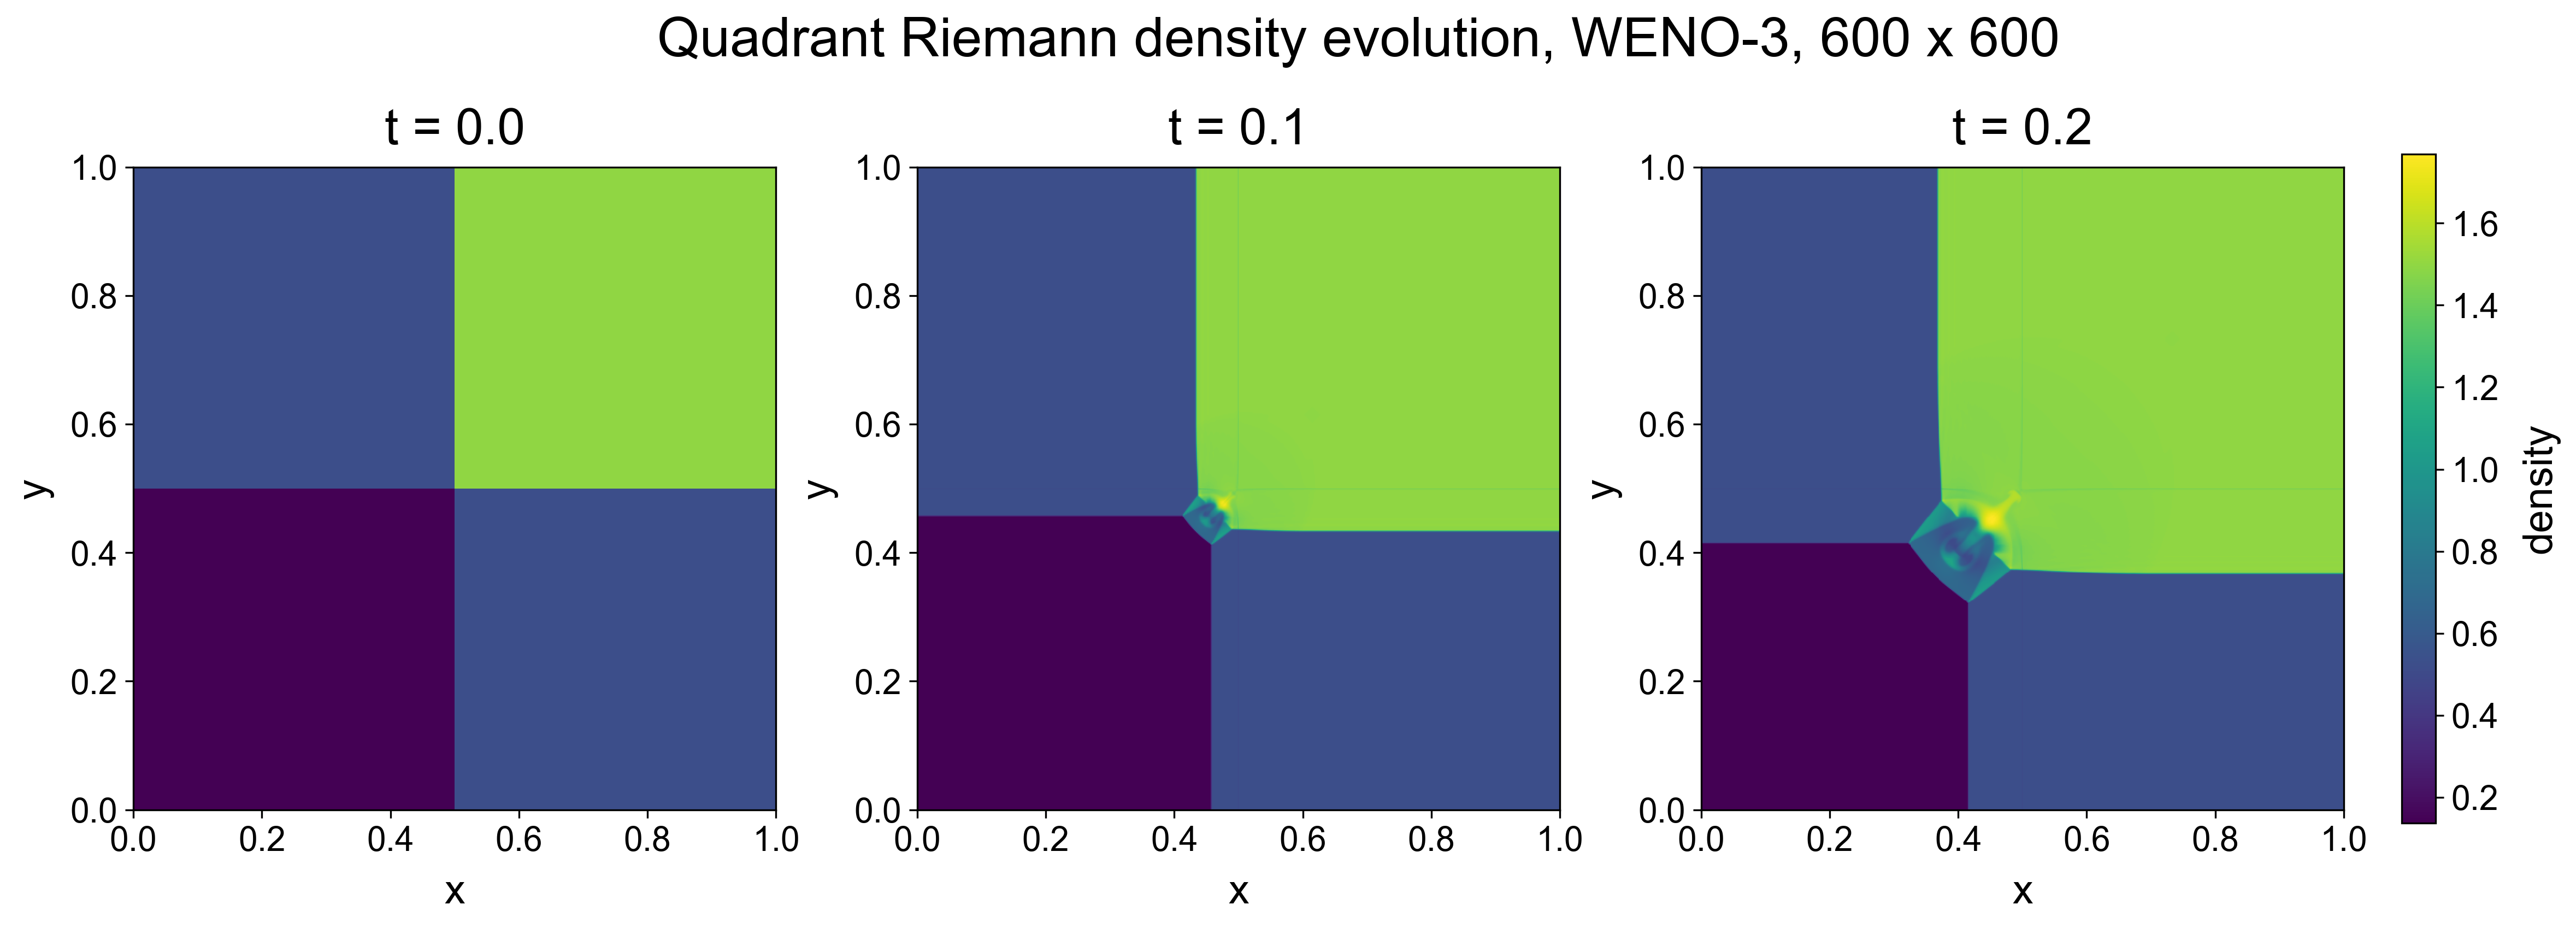
\includegraphics[width=0.98\textwidth]{quadrant_riemann_weno3_evolution_n600.png}
\caption{Density evolution in the \(600\times600\) HLLC WENO-3 quadrant Riemann
calculation. A common colour scale is used at \(t=0\), \(0.1\), and \(0.2\).}
\label{fig:quadrant-evolution-discontinuous}
\end{figure}

Figure~\ref{fig:quadrant-evolution-discontinuous} establishes the temporal development.
Figure~\ref{fig:quadrant-fields-discontinuous} then fixes the final time and colour scale
to compare method-dependent interface thickness and local extrema.

\begin{figure}[!htbp]
\centering
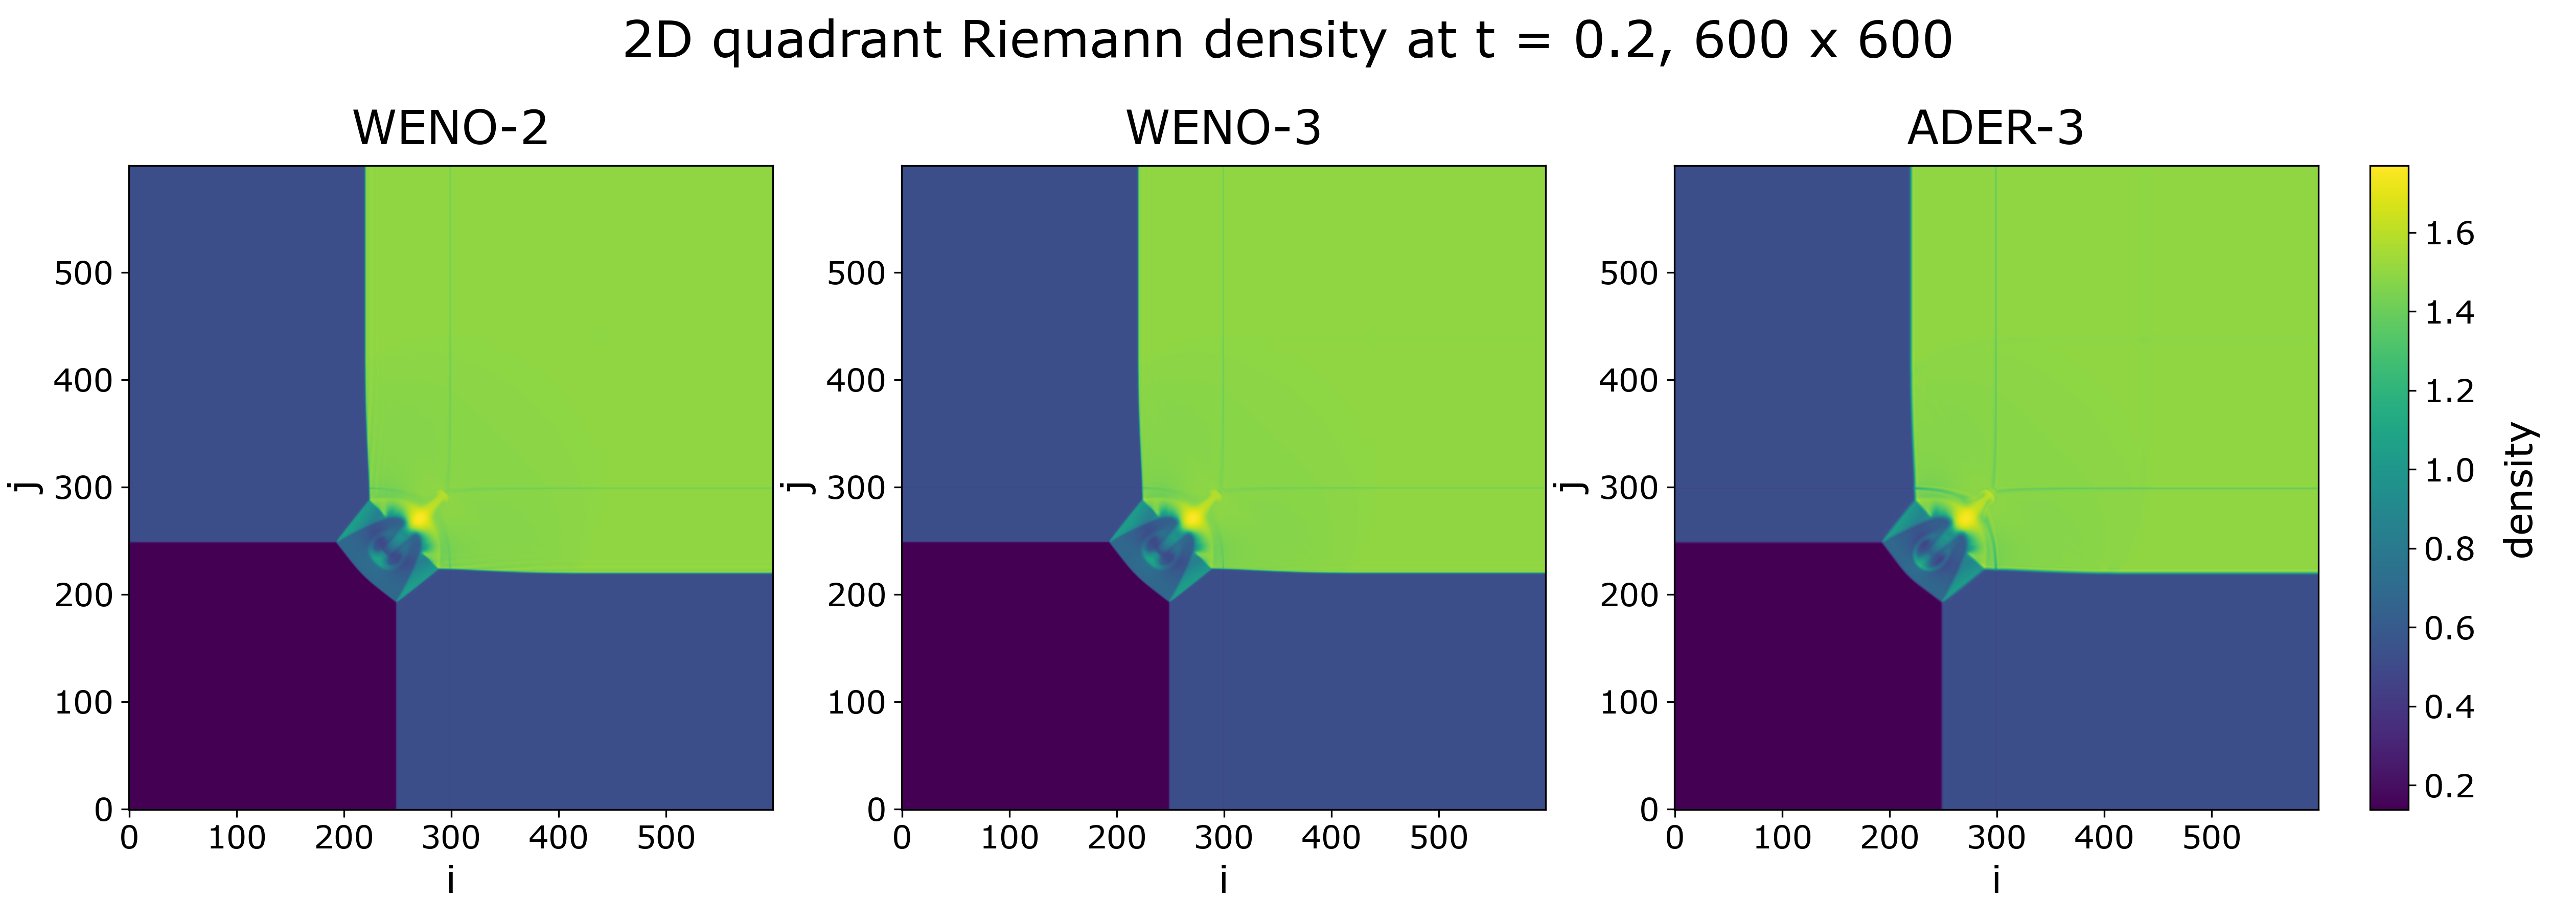
\includegraphics[width=0.98\textwidth]{quadrant_riemann_hllc_n600.png}
\caption{Quadrant Riemann density at \(t=0.2\) and \(600\times600\). Each panel uses
the same colour scale. All methods preserve the four far-field states and resolve the same
large-scale wave pattern. Their differences are concentrated near the compact interaction
region.}
\label{fig:quadrant-fields-discontinuous}
\end{figure}

The three final fields preserve the four far-field states and the same interacting-wave
topology, while their visible differences remain confined to the compact central region.
The off-interface slice in Figure~\ref{fig:quadrant-slice-discontinuous} then gives a more
discriminating comparison: the main jump, intermediate trough and post-interaction plateau
occur at the same coordinates for all three methods.

\begin{figure}[!htbp]
\centering
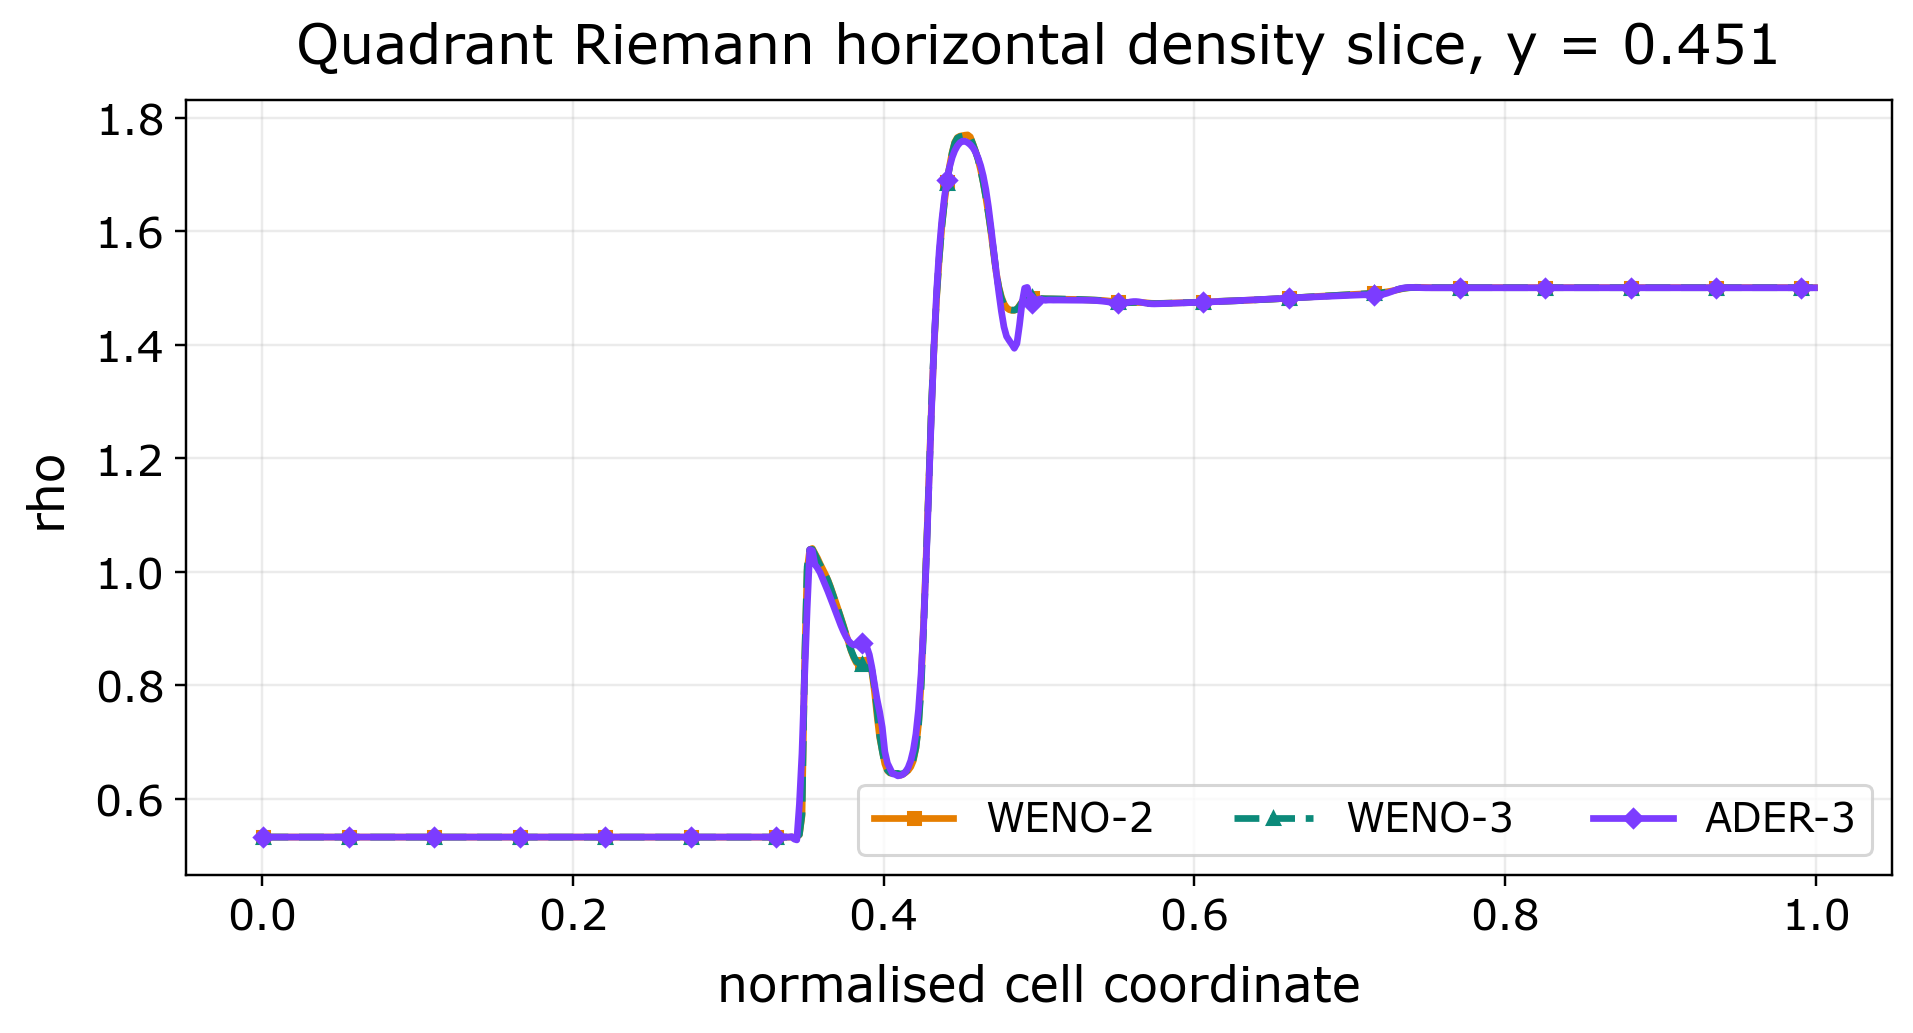
\includegraphics[width=0.90\textwidth]{quadrant_riemann_slice_hllc_n600.png}
\caption{Quadrant Riemann density along \(y=0.451\). Sampling away from the initial
quadrant boundary removes cell-ownership ambiguity while retaining the interacting waves.}
\label{fig:quadrant-slice-discontinuous}
\end{figure}

WENO-3 follows WENO-2 closely but resolves the narrow changes more steeply. ADER-3
captures the same state sequence with a stronger local excursion near the interaction,
where its troubled-interface decision switches between the space--time predictor and
cell-average HLLC fallback. The flat states away from the waves show that these are local
method differences, not an incorrect initial condition. Figure~\ref{fig:third-order-quadrant-difference}
next localises the still smaller backend discrepancies relative to that common solution.

WENO-3 remains near roundoff in energy, whereas the dominant ADER-3
\(x\)-velocity discrepancy reaches $3.679\times10^{-12}$. In both maps the largest
local values follow the discontinuities and central interaction region, where small
backend perturbations encounter the steepest reconstructed gradients.

The WENO-3 map also has a nearly uniform background in the upper-right far-field state.
Its mean energy difference there is approximately \(3.1\times10^{-14}\), compared with
\(2.1\times10^{-16}\) in the lower-left far field. Because the upper-right state has the
largest total-energy magnitude, a higher absolute roundoff floor is expected. The plateau
contains no displaced-wave pattern, while the brighter lines identify local amplification
near discontinuities. Neither feature indicates an incorrect initial condition or a
domain-wide physical displacement.

\begin{figure}[!htbp]
\centering
\begin{subfigure}[t]{0.47\textwidth}
\centering
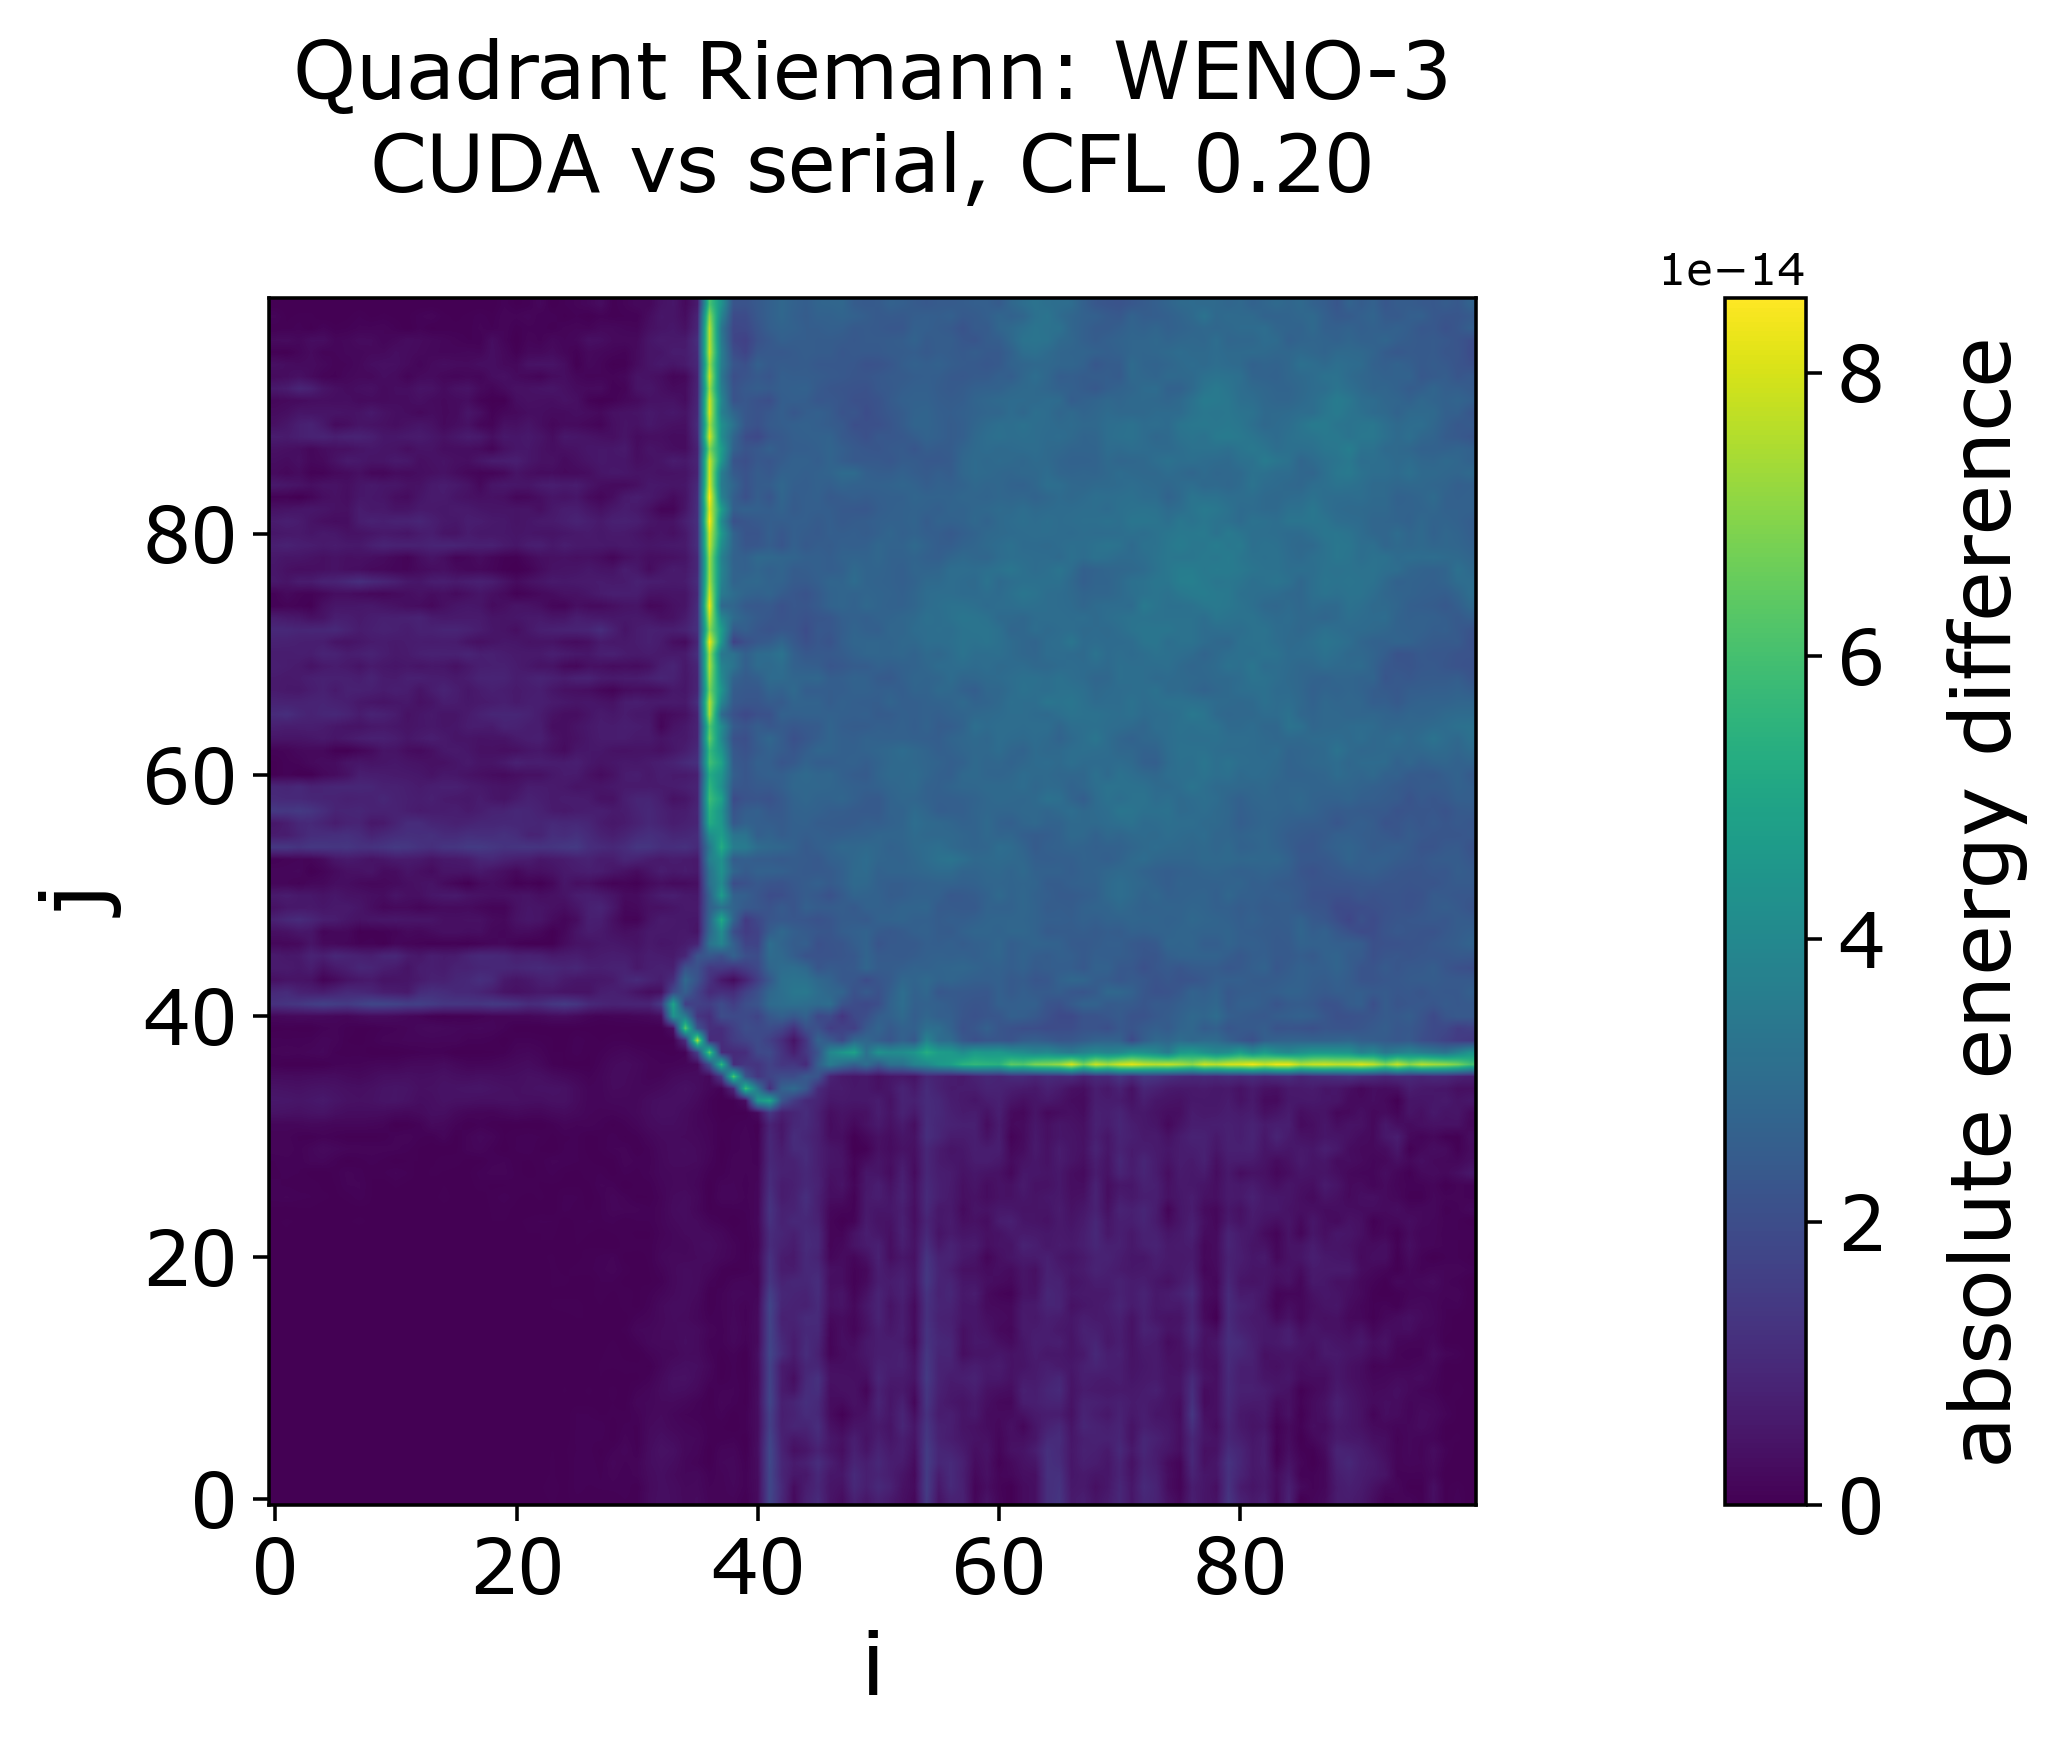
\includegraphics[width=\linewidth]{quadrant_riemann_weno3_energy_absdiff_cfl020.png}
\caption{WENO-3, CFL 0.20: $\max|\Delta E|=8.527\times10^{-14}$.}
\end{subfigure}\hfill
\begin{subfigure}[t]{0.47\textwidth}
\centering
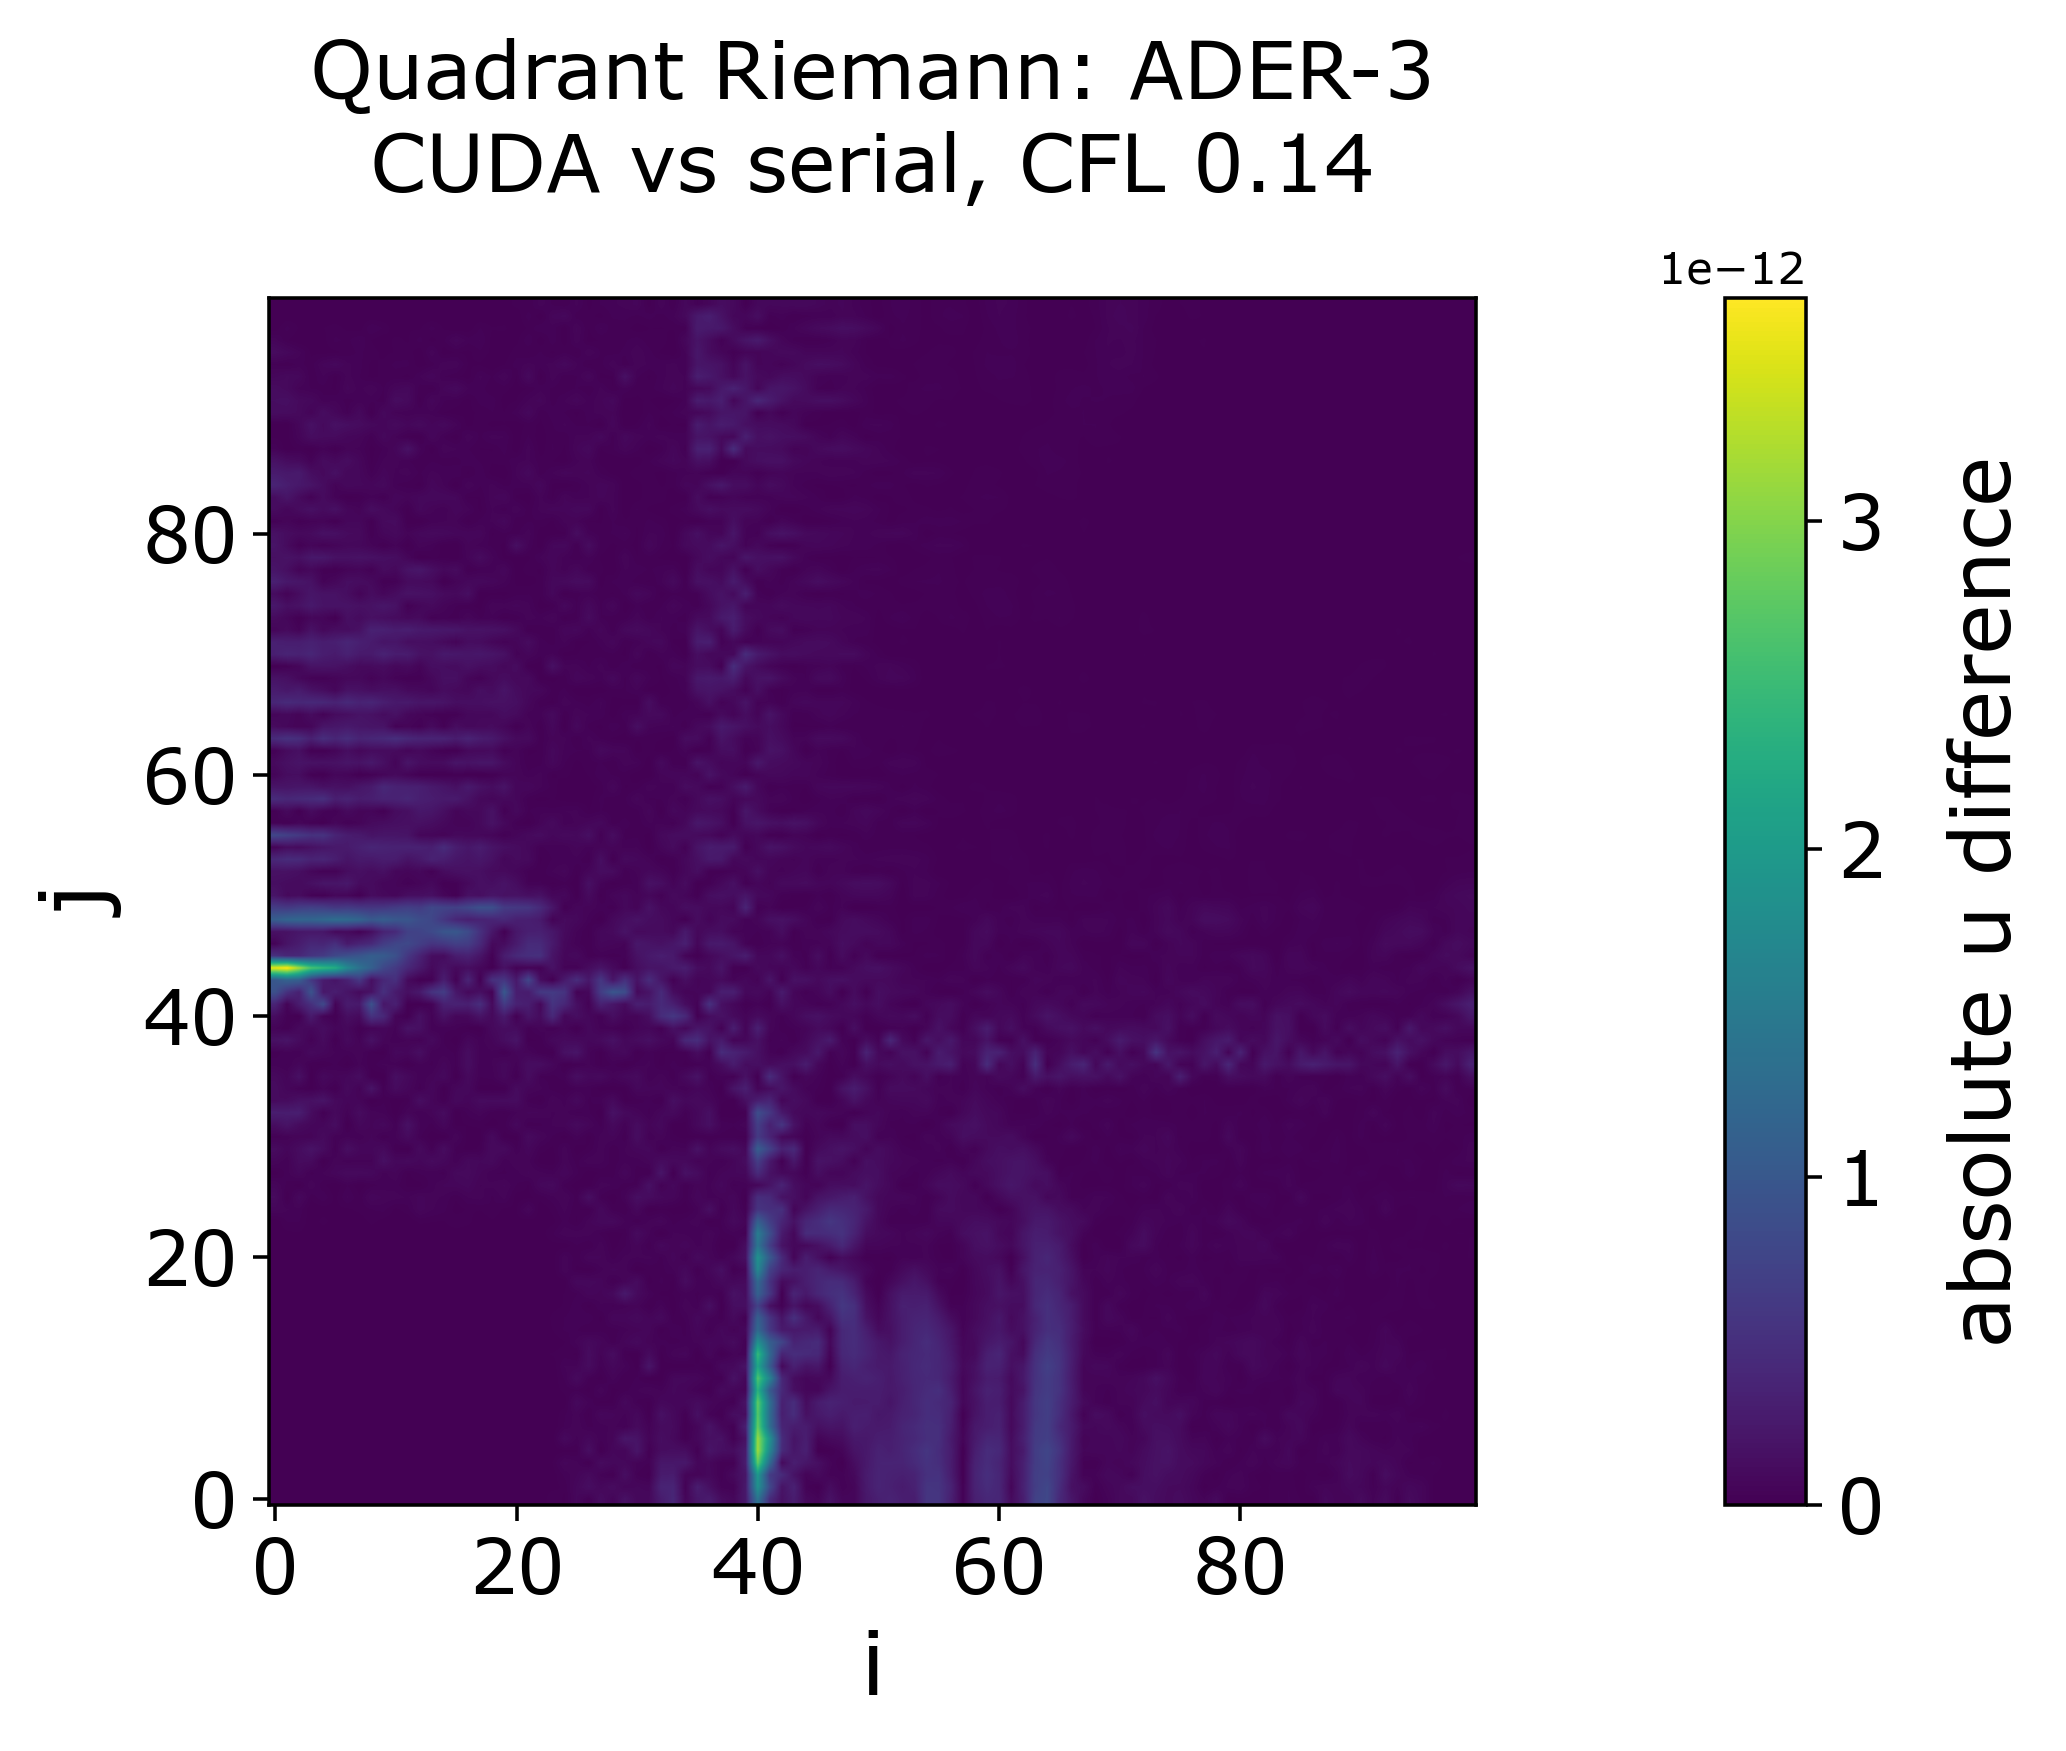
\includegraphics[width=\linewidth]{quadrant_riemann_ader3_u_absdiff_cfl014.png}
\caption{ADER-3, CFL 0.14: $\max|\Delta u|=3.679\times10^{-12}$.}
\end{subfigure}
\caption{Absolute CUDA--serial differences for the quadrant Riemann problem at
$100\times100$. The plotted variable is the dominant field for each method and each panel
uses its own colour scale.}
\label{fig:third-order-quadrant-difference}
\end{figure}

\FloatBarrier
\subsection*{Shock--bubble interaction}

This test is especially relevant to HLLC because the low-density bubble is bounded by a
curved contact. Figure~\ref{fig:shock-evolution-discontinuous} separates the main stages:
a planar shock approaches the bubble at \(t=0\), enters and deforms it by \(t=0.1\), and
leaves reflected and transmitted waves around a distorted low-density region at \(t=0.2\).

\begin{figure}[!htbp]
\centering
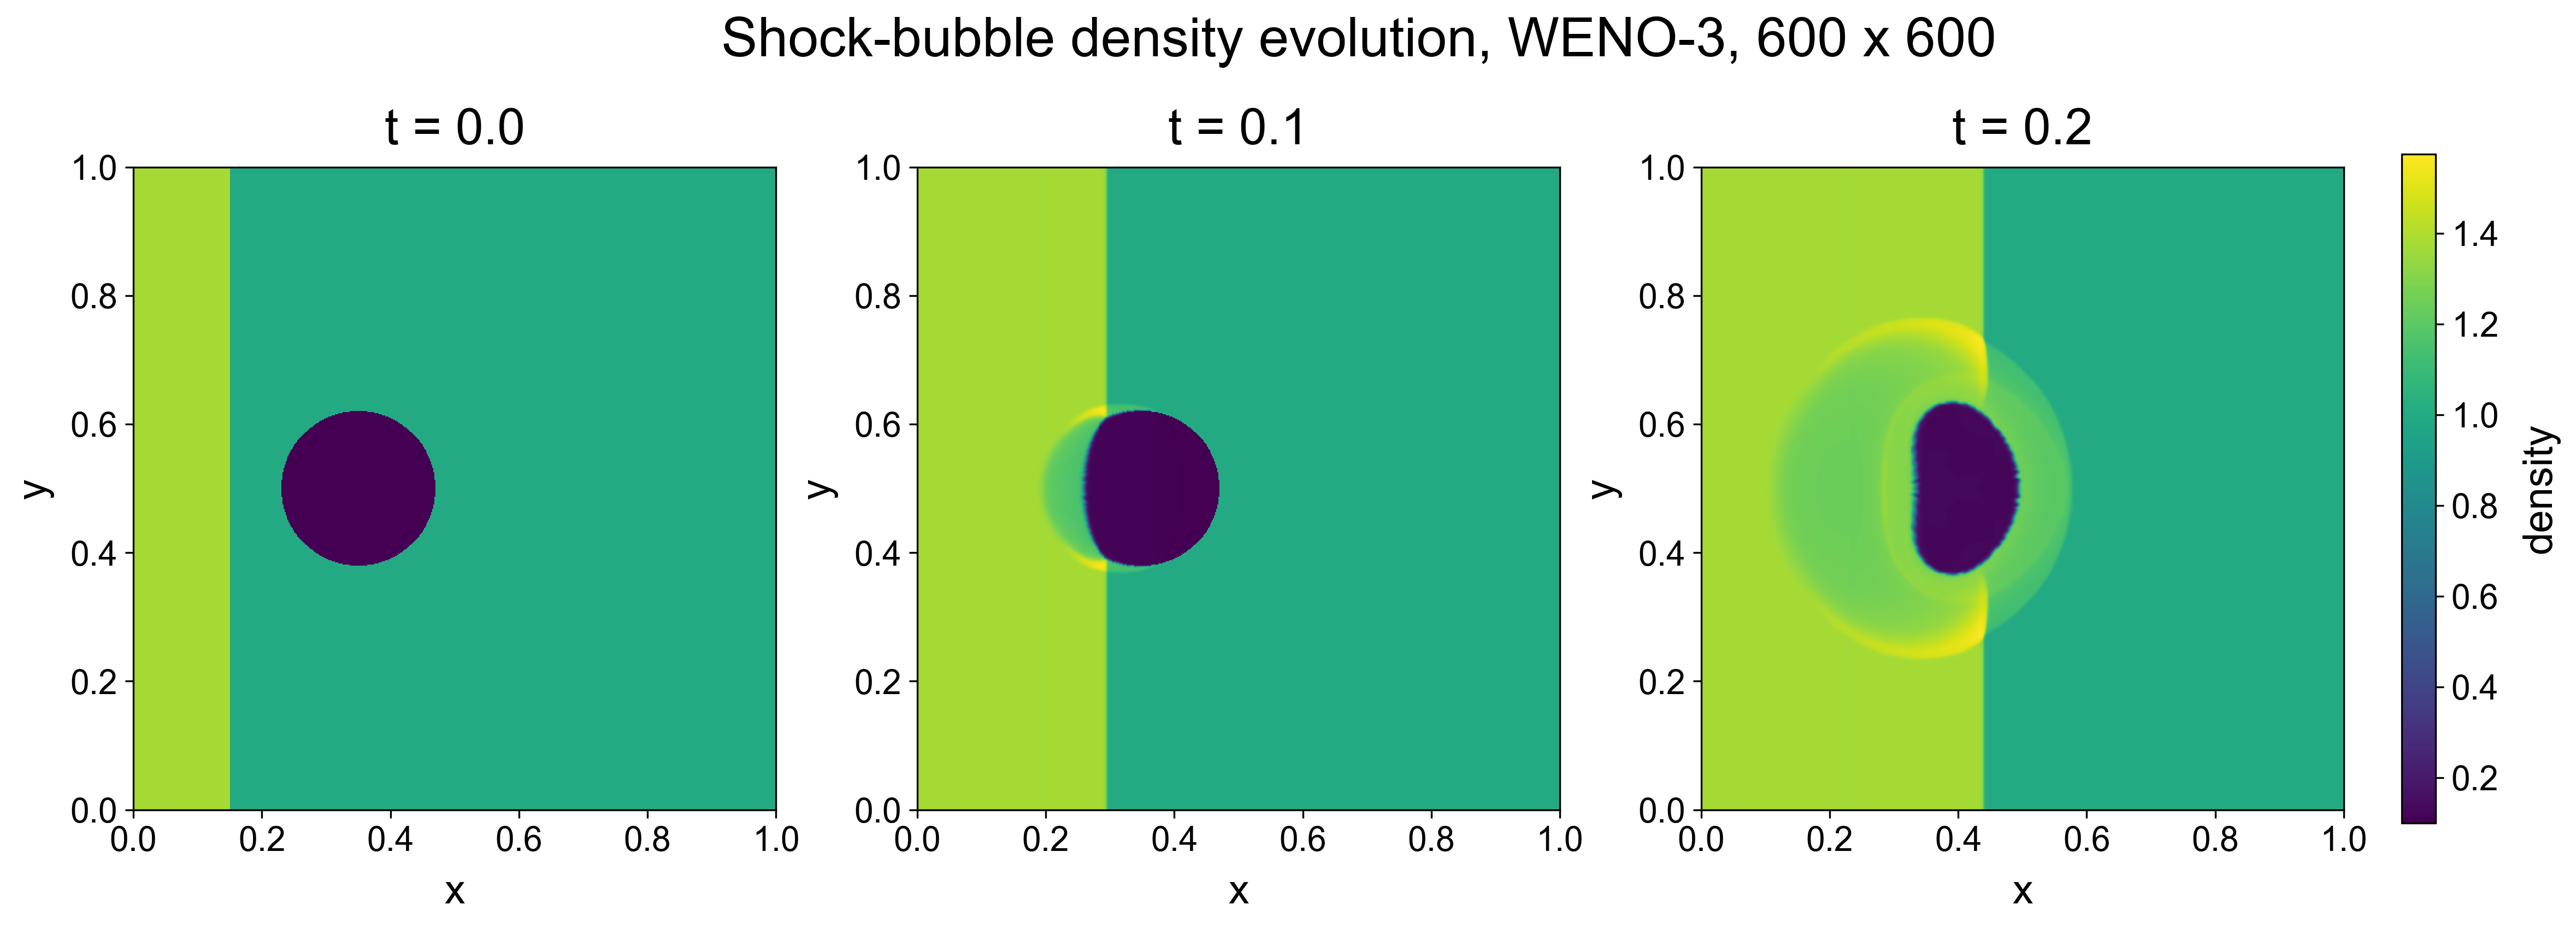
\includegraphics[width=0.98\textwidth]{shock_bubble_weno3_evolution_n600.png}
\caption{Density evolution in the \(600\times600\) HLLC WENO-3 shock--bubble
calculation. The panels at \(t=0\), \(0.1\), and \(0.2\) use one common colour scale.}
\label{fig:shock-evolution-discontinuous}
\end{figure}

The evolution sequence identifies approach, impact and post-interaction deformation.
Figure~\ref{fig:shock-fields-discontinuous} then fixes \(t=0.2\) and the colour scale to
compare numerical diffusion and contact resolution across the three methods.

\begin{figure}[!htbp]
\centering
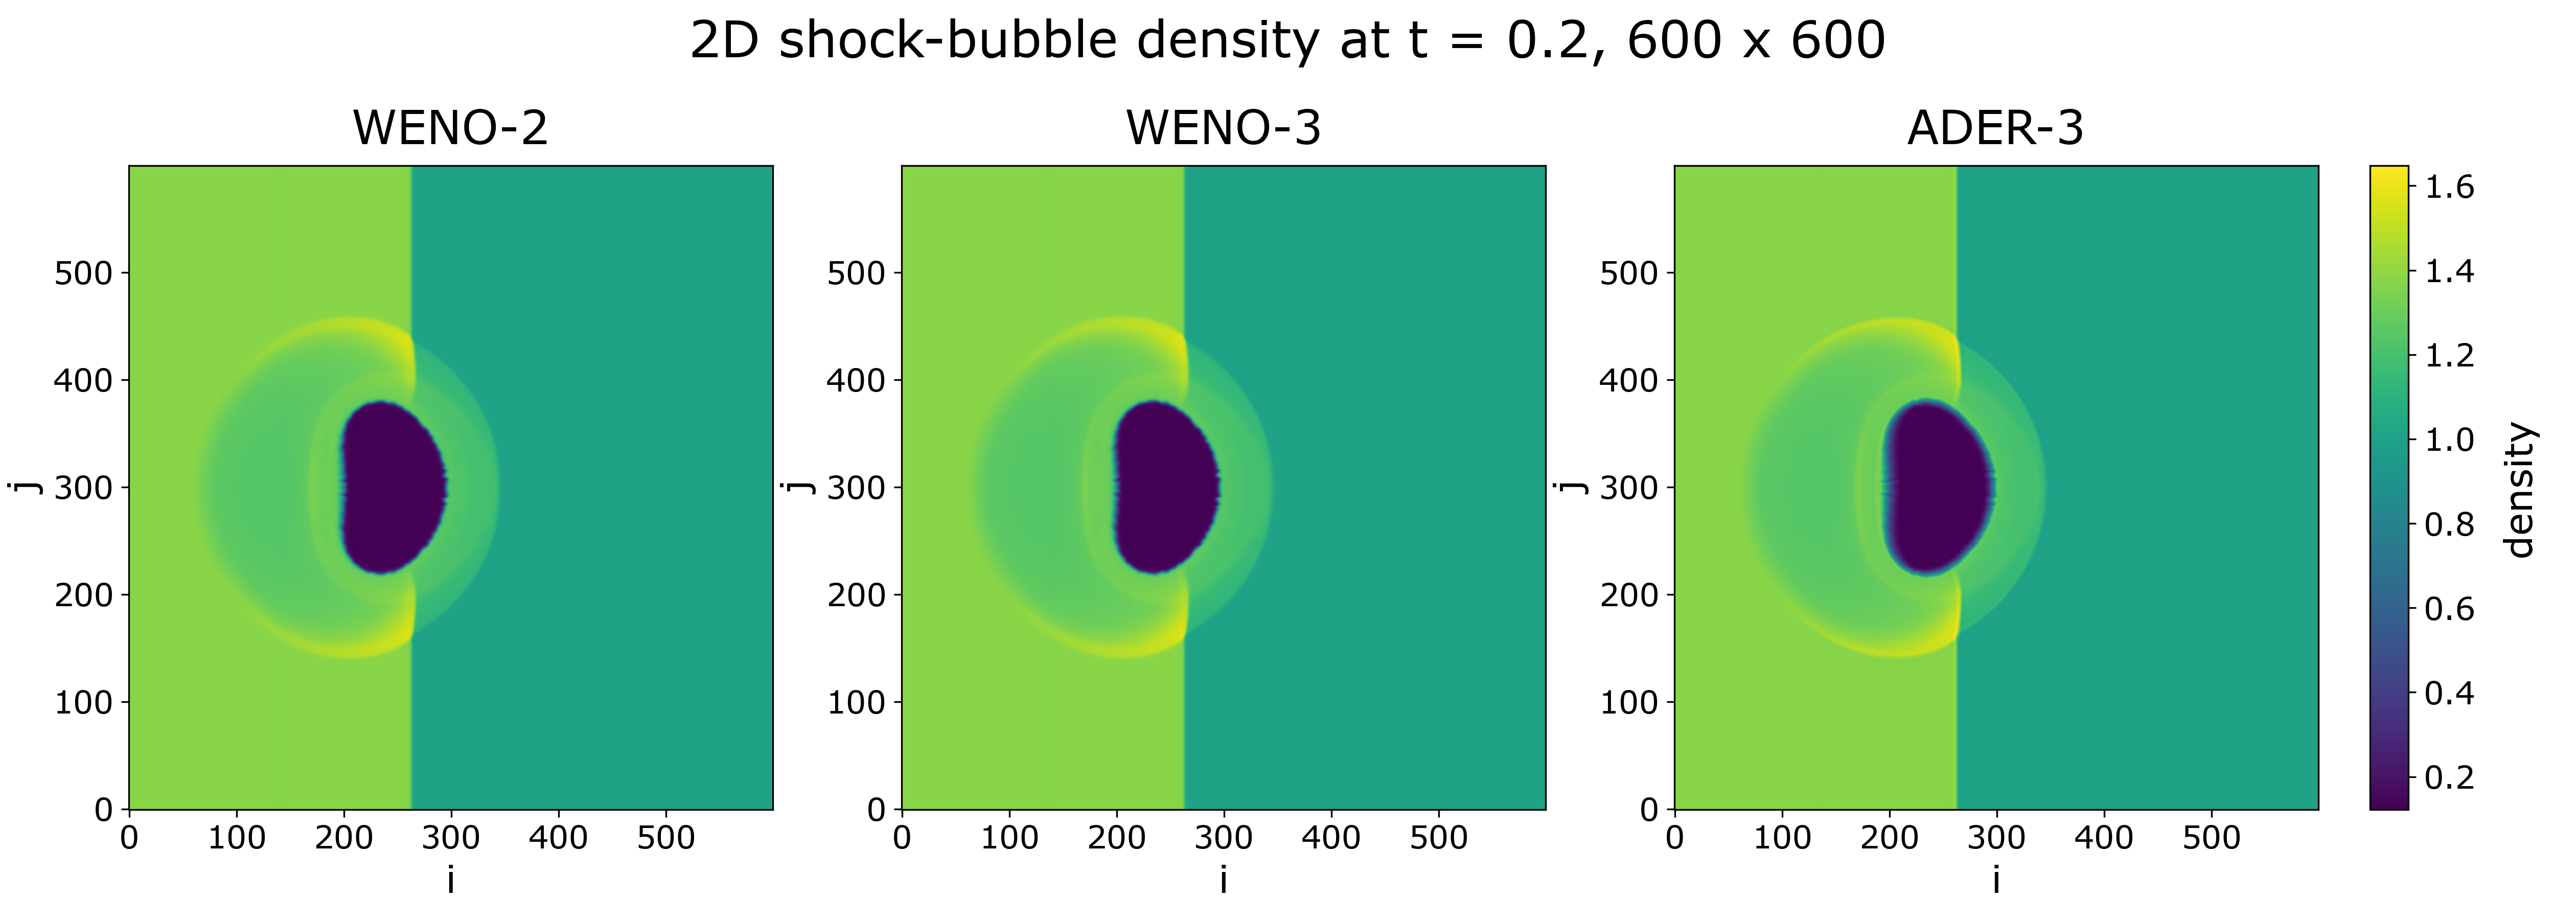
\includegraphics[width=0.98\textwidth]{shock_bubble_hllc_n600.png}
\caption{Shock--bubble density at \(t=0.2\) and \(600\times600\). The shared colour
scale exposes differences in contact thickness and extrema around the curved bubble:
WENO-2 is the most diffusive, WENO-3 retains a thinner transition, and ADER-3 gives the
strongest local contrast.}
\label{fig:shock-fields-discontinuous}
\end{figure}

All three final fields propagate the incident shock through the bubble and preserve the
expected distorted low-density region. Their differences are concentrated in contact
thickness and nearby extrema, as the centre-near slice in
Figure~\ref{fig:shock-slice-discontinuous} makes explicit.

\begin{figure}[!htbp]
\centering
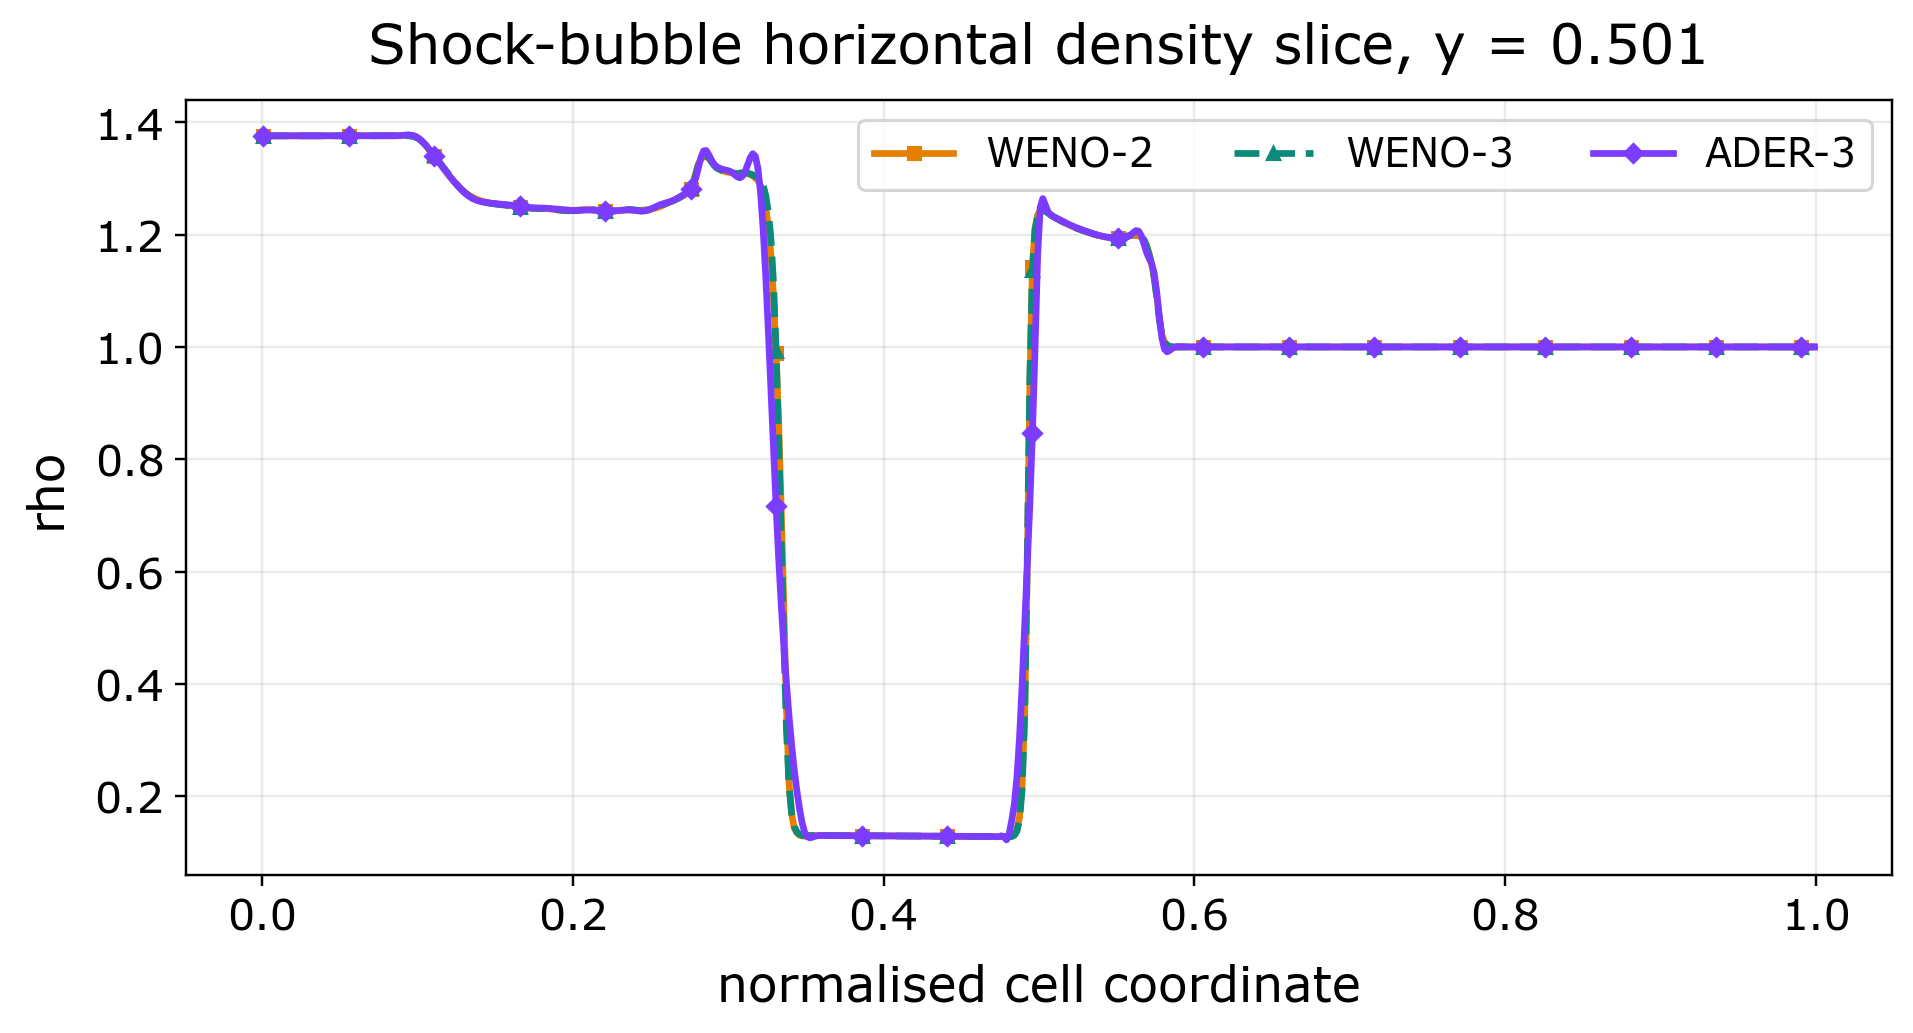
\includegraphics[width=0.90\textwidth]{shock_bubble_slice_hllc_n600.png}
\caption{Shock--bubble density along \(y=0.501\). All cell values contribute to each
line, while markers are thinned for readability.}
\label{fig:shock-slice-discontinuous}
\end{figure}

The three profiles agree through the post-shock and undisturbed states. WENO-2 gives the
broadest bubble boundaries, WENO-3 retains thinner transitions, and ADER-3 produces the
strongest local contrast. Its less smooth edge is confined to the curved interface, where
the Cartesian representation and troubled-interface fallback are most active. It is not
a global background-state error. Figure~\ref{fig:third-order-shock-difference} then tests
whether backend discrepancies alter this resolved flow or remain local.

The WENO-3 map has a visibly layered background. Its mean energy difference is
approximately \(5.2\times10^{-14}\) in the post-shock region on the left and
\(2.7\times10^{-15}\) in the undisturbed right region. These layers follow states of
different magnitude and accumulated arithmetic, while the complete map remains at
roundoff scale with a maximum of \(7.860\times10^{-14}\).

\begin{figure}[!htbp]
\centering
\begin{subfigure}[t]{0.47\textwidth}
\centering
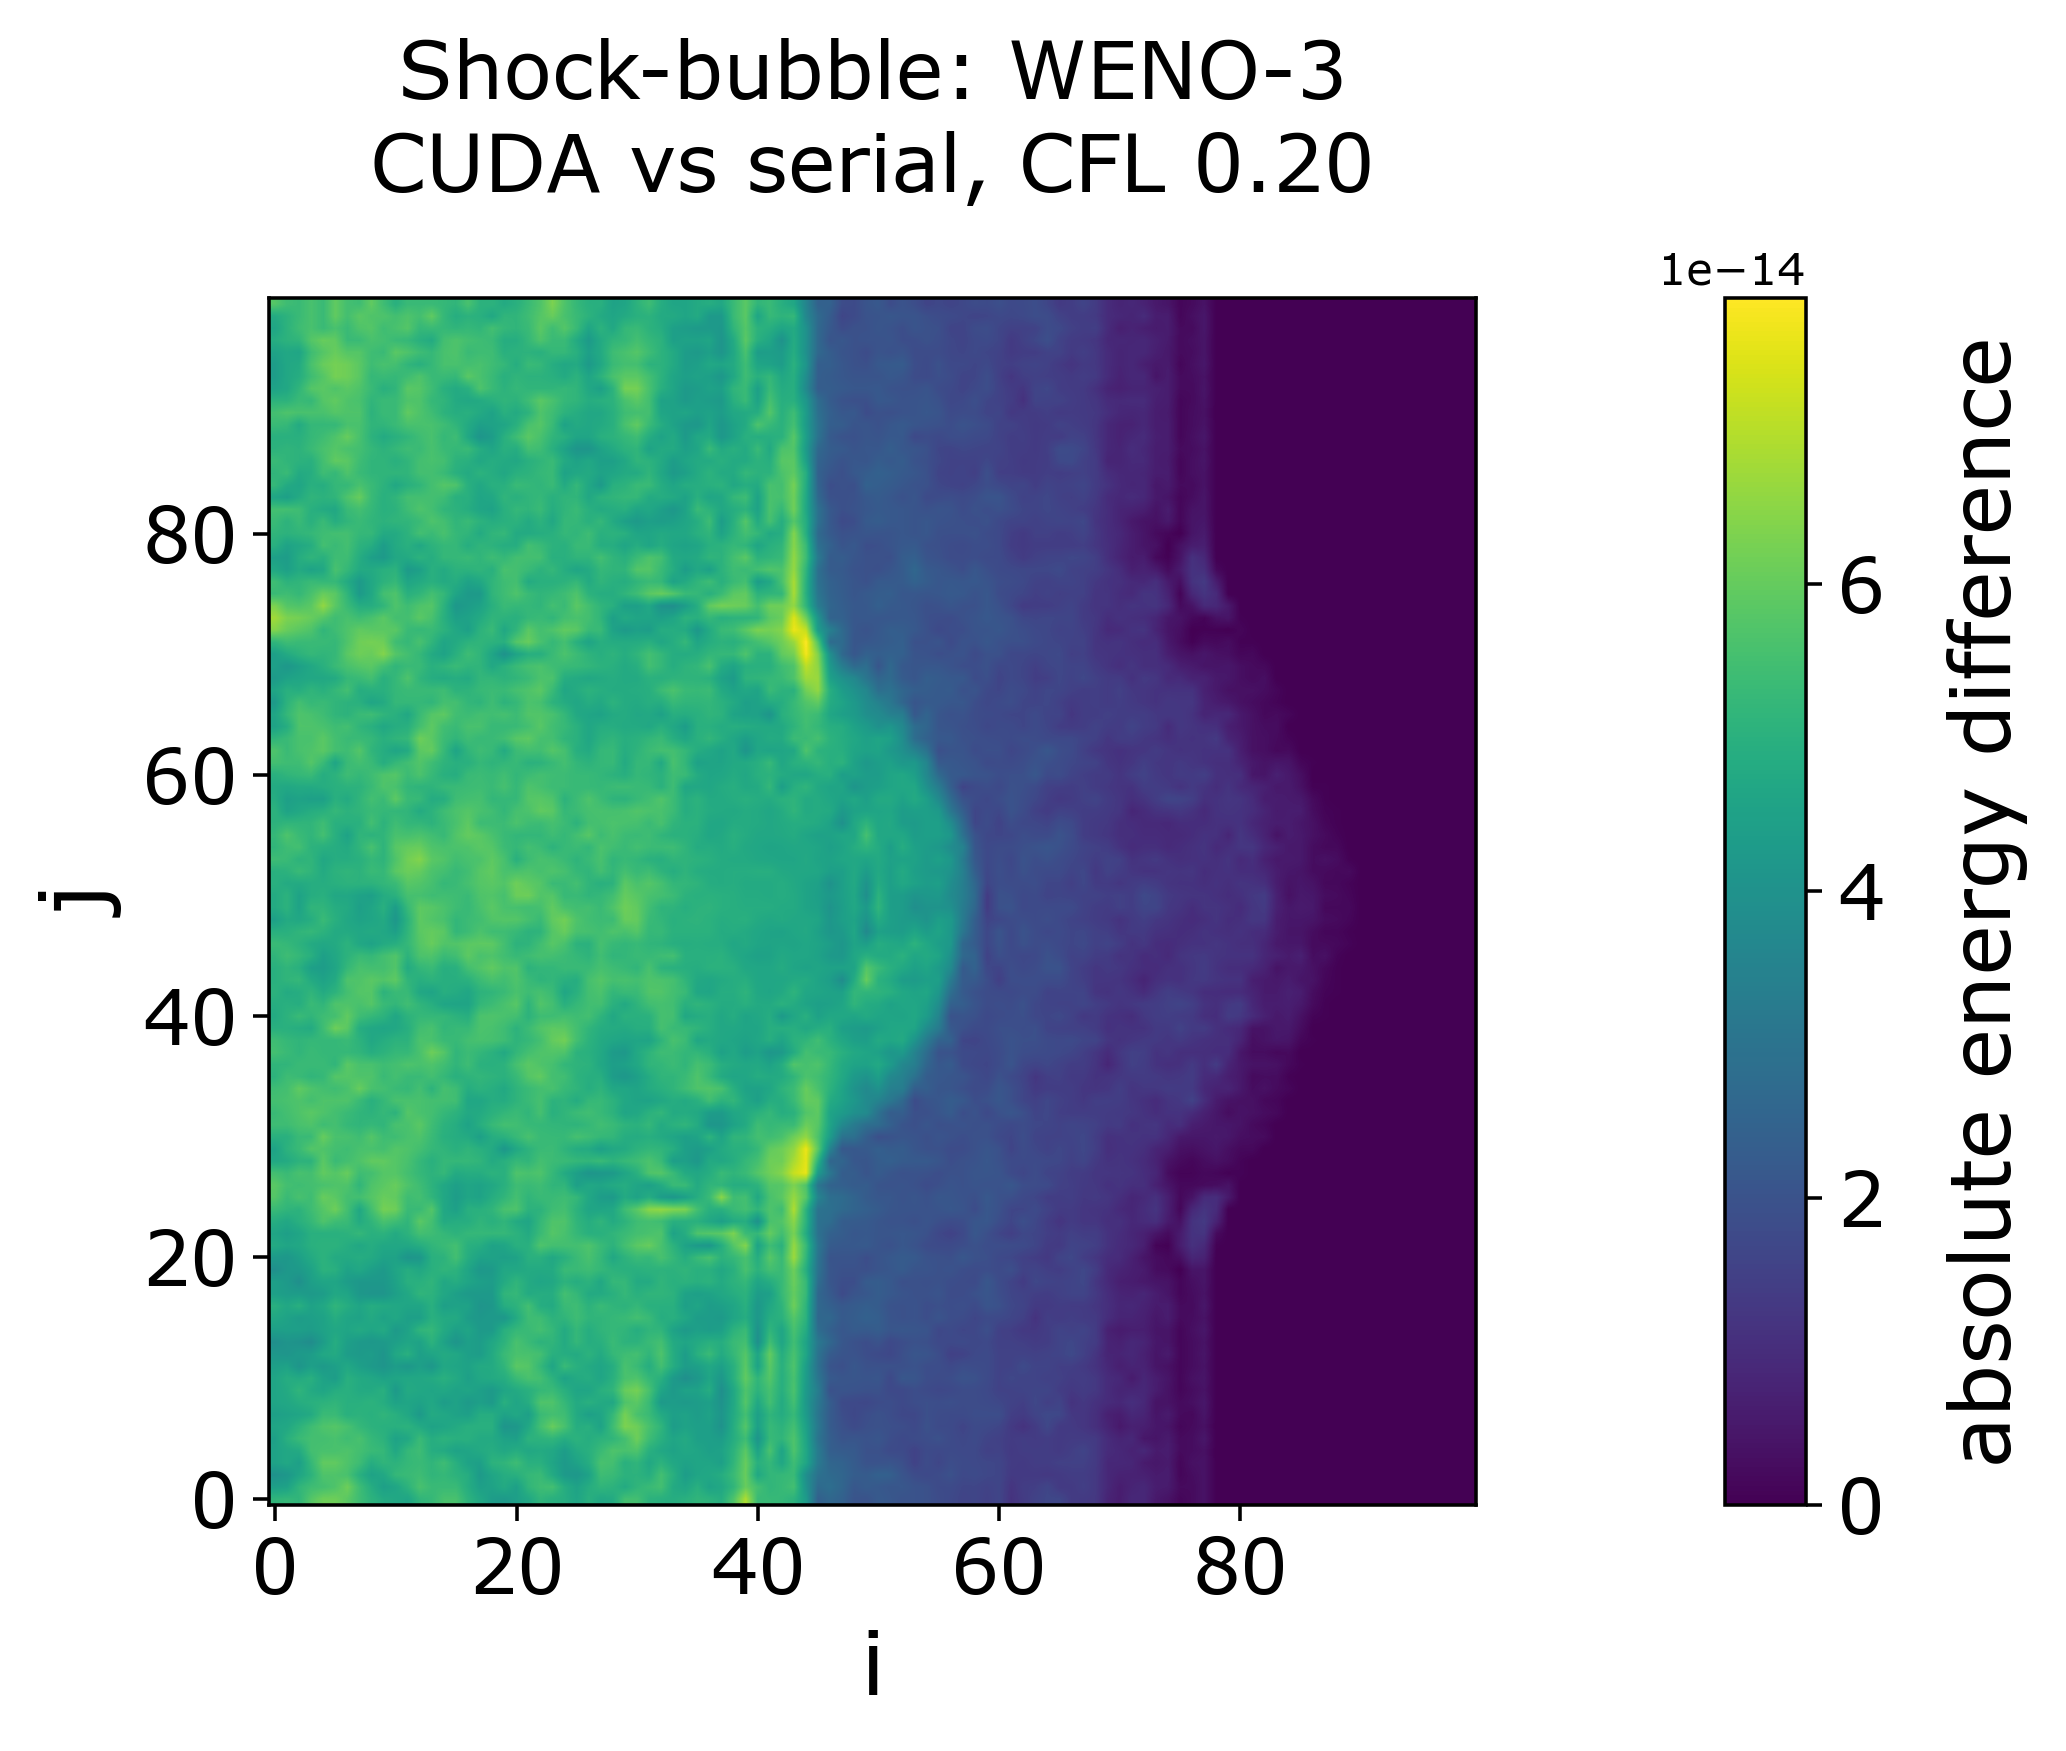
\includegraphics[width=\linewidth]{shock_bubble_weno3_energy_absdiff_cfl020.png}
\caption{WENO-3, CFL 0.20: $\max|\Delta E|=7.860\times10^{-14}$.}
\end{subfigure}\hfill
\begin{subfigure}[t]{0.47\textwidth}
\centering
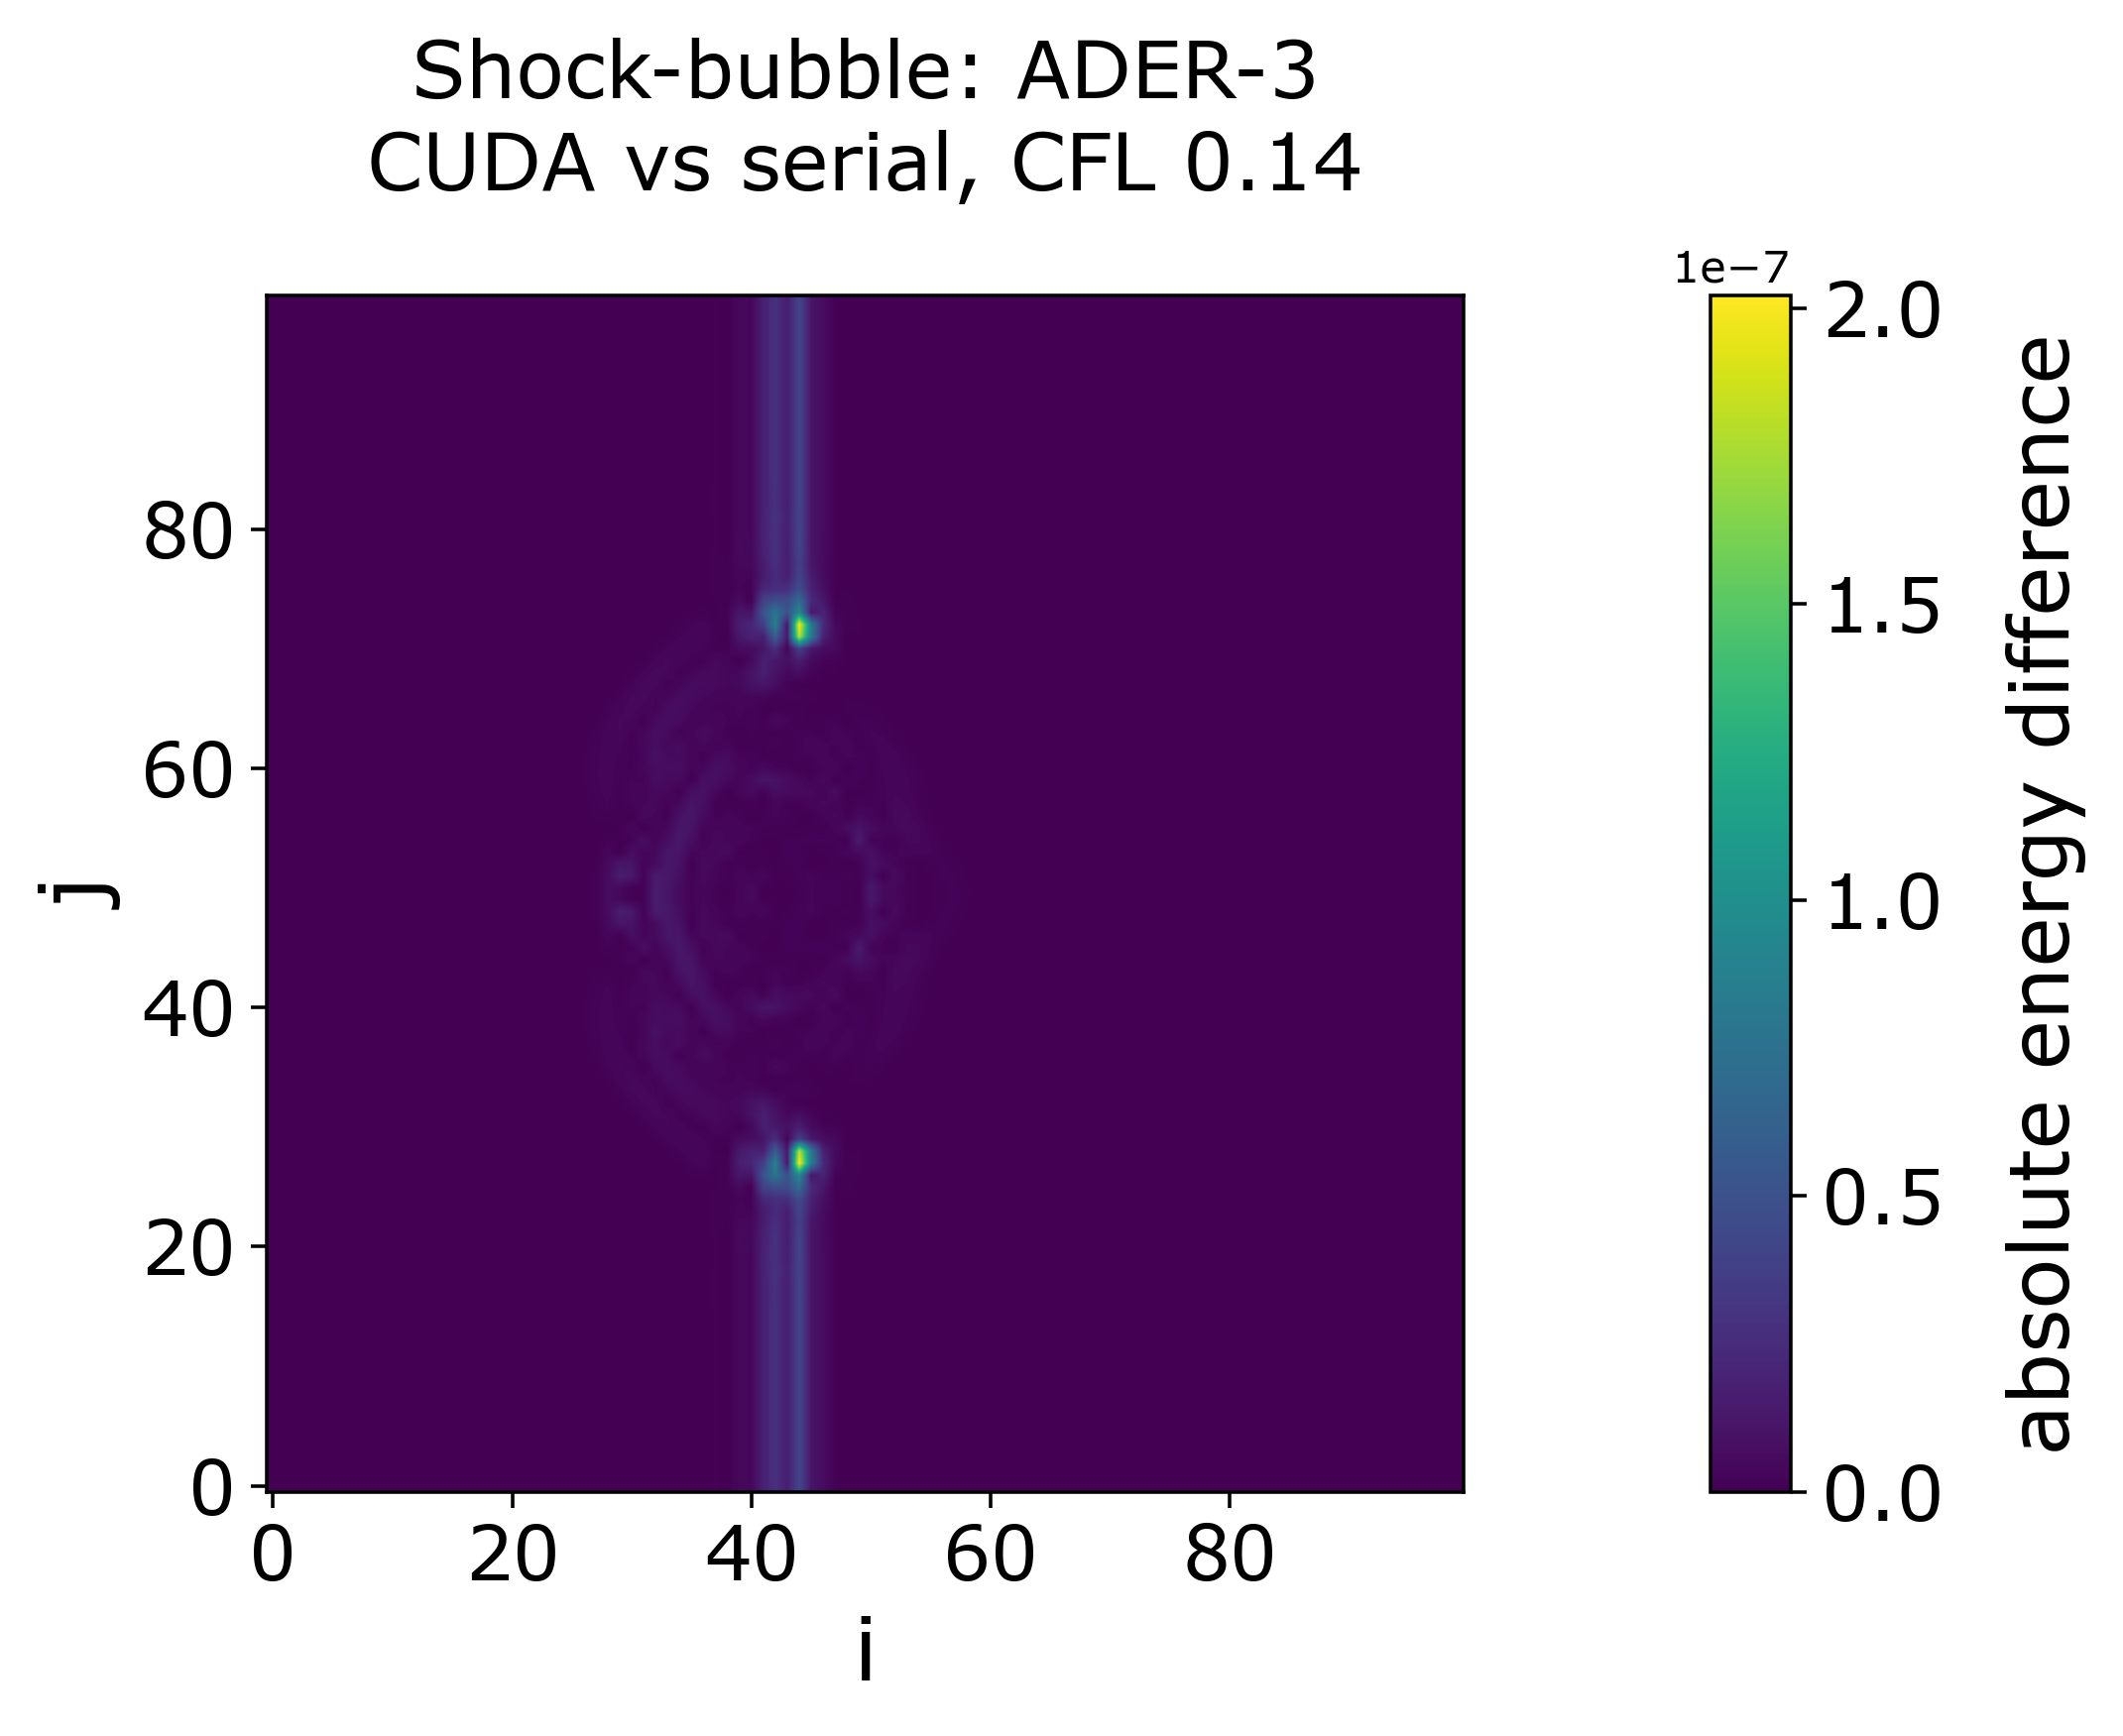
\includegraphics[width=\linewidth]{shock_bubble_ader3_energy_absdiff_cfl014.png}
\caption{ADER-3, CFL 0.14: $\max|\Delta E|=2.021\times10^{-7}$.}
\end{subfigure}
\caption{Absolute CUDA--serial energy differences for the shock--bubble problem at
\(100\times100\). WENO-3 shows broad state-dependent layers at roundoff scale, whereas
ADER-3 is dominated by local peaks where the moving front meets the bubble boundary.
Each panel uses its own colour scale.}
\label{fig:third-order-shock-difference}
\end{figure}

ADER-3 has a more localised signature. Its darker background is interrupted along the
moving shock/contact structure and the faint curved bubble interface. The two strongest
peaks occur near \((i,j)=(44,27)\) and \((44,72)\), where the front intersects the lower
and upper bubble boundaries, and reach \(2.021\times10^{-7}\). They are consistent with
the troubled-interface and fallback sensitivity discussed below, not with displacement of
the complete bubble or shock.

\begin{table}[H]
\centering
\small
\begin{tabular}{llrl}
\toprule
Problem & Method & CUDA maximum difference & Dominant field \\
\midrule
Gaussian advection & WENO-2 & \(3.997\times10^{-15}\) & \(E\) \\
Gaussian advection & WENO-3 & \(8.438\times10^{-15}\) & \(E\) \\
Gaussian advection & ADER-3 & \(2.445\times10^{-12}\) & \(E\) \\
Quadrant Riemann & WENO-2 & \(1.310\times10^{-14}\) & \(v\) \\
Quadrant Riemann & WENO-3 & \(8.527\times10^{-14}\) & \(E\) \\
Quadrant Riemann & ADER-3 & \(3.679\times10^{-12}\) & \(u\) \\
Shock--bubble & WENO-2 & \(1.865\times10^{-14}\) & \(E\) \\
Shock--bubble & WENO-3 & \(7.860\times10^{-14}\) & \(E\) \\
Shock--bubble & ADER-3 & \(2.021\times10^{-7}\) & \(E\) \\
\bottomrule
\end{tabular}
\caption{Maximum absolute field difference against serial at \(100\times100\). OpenMP differences are zero in every exported field.}
\label{tab:backend-diff}
\end{table}

\begin{figure}[!htbp]
\centering
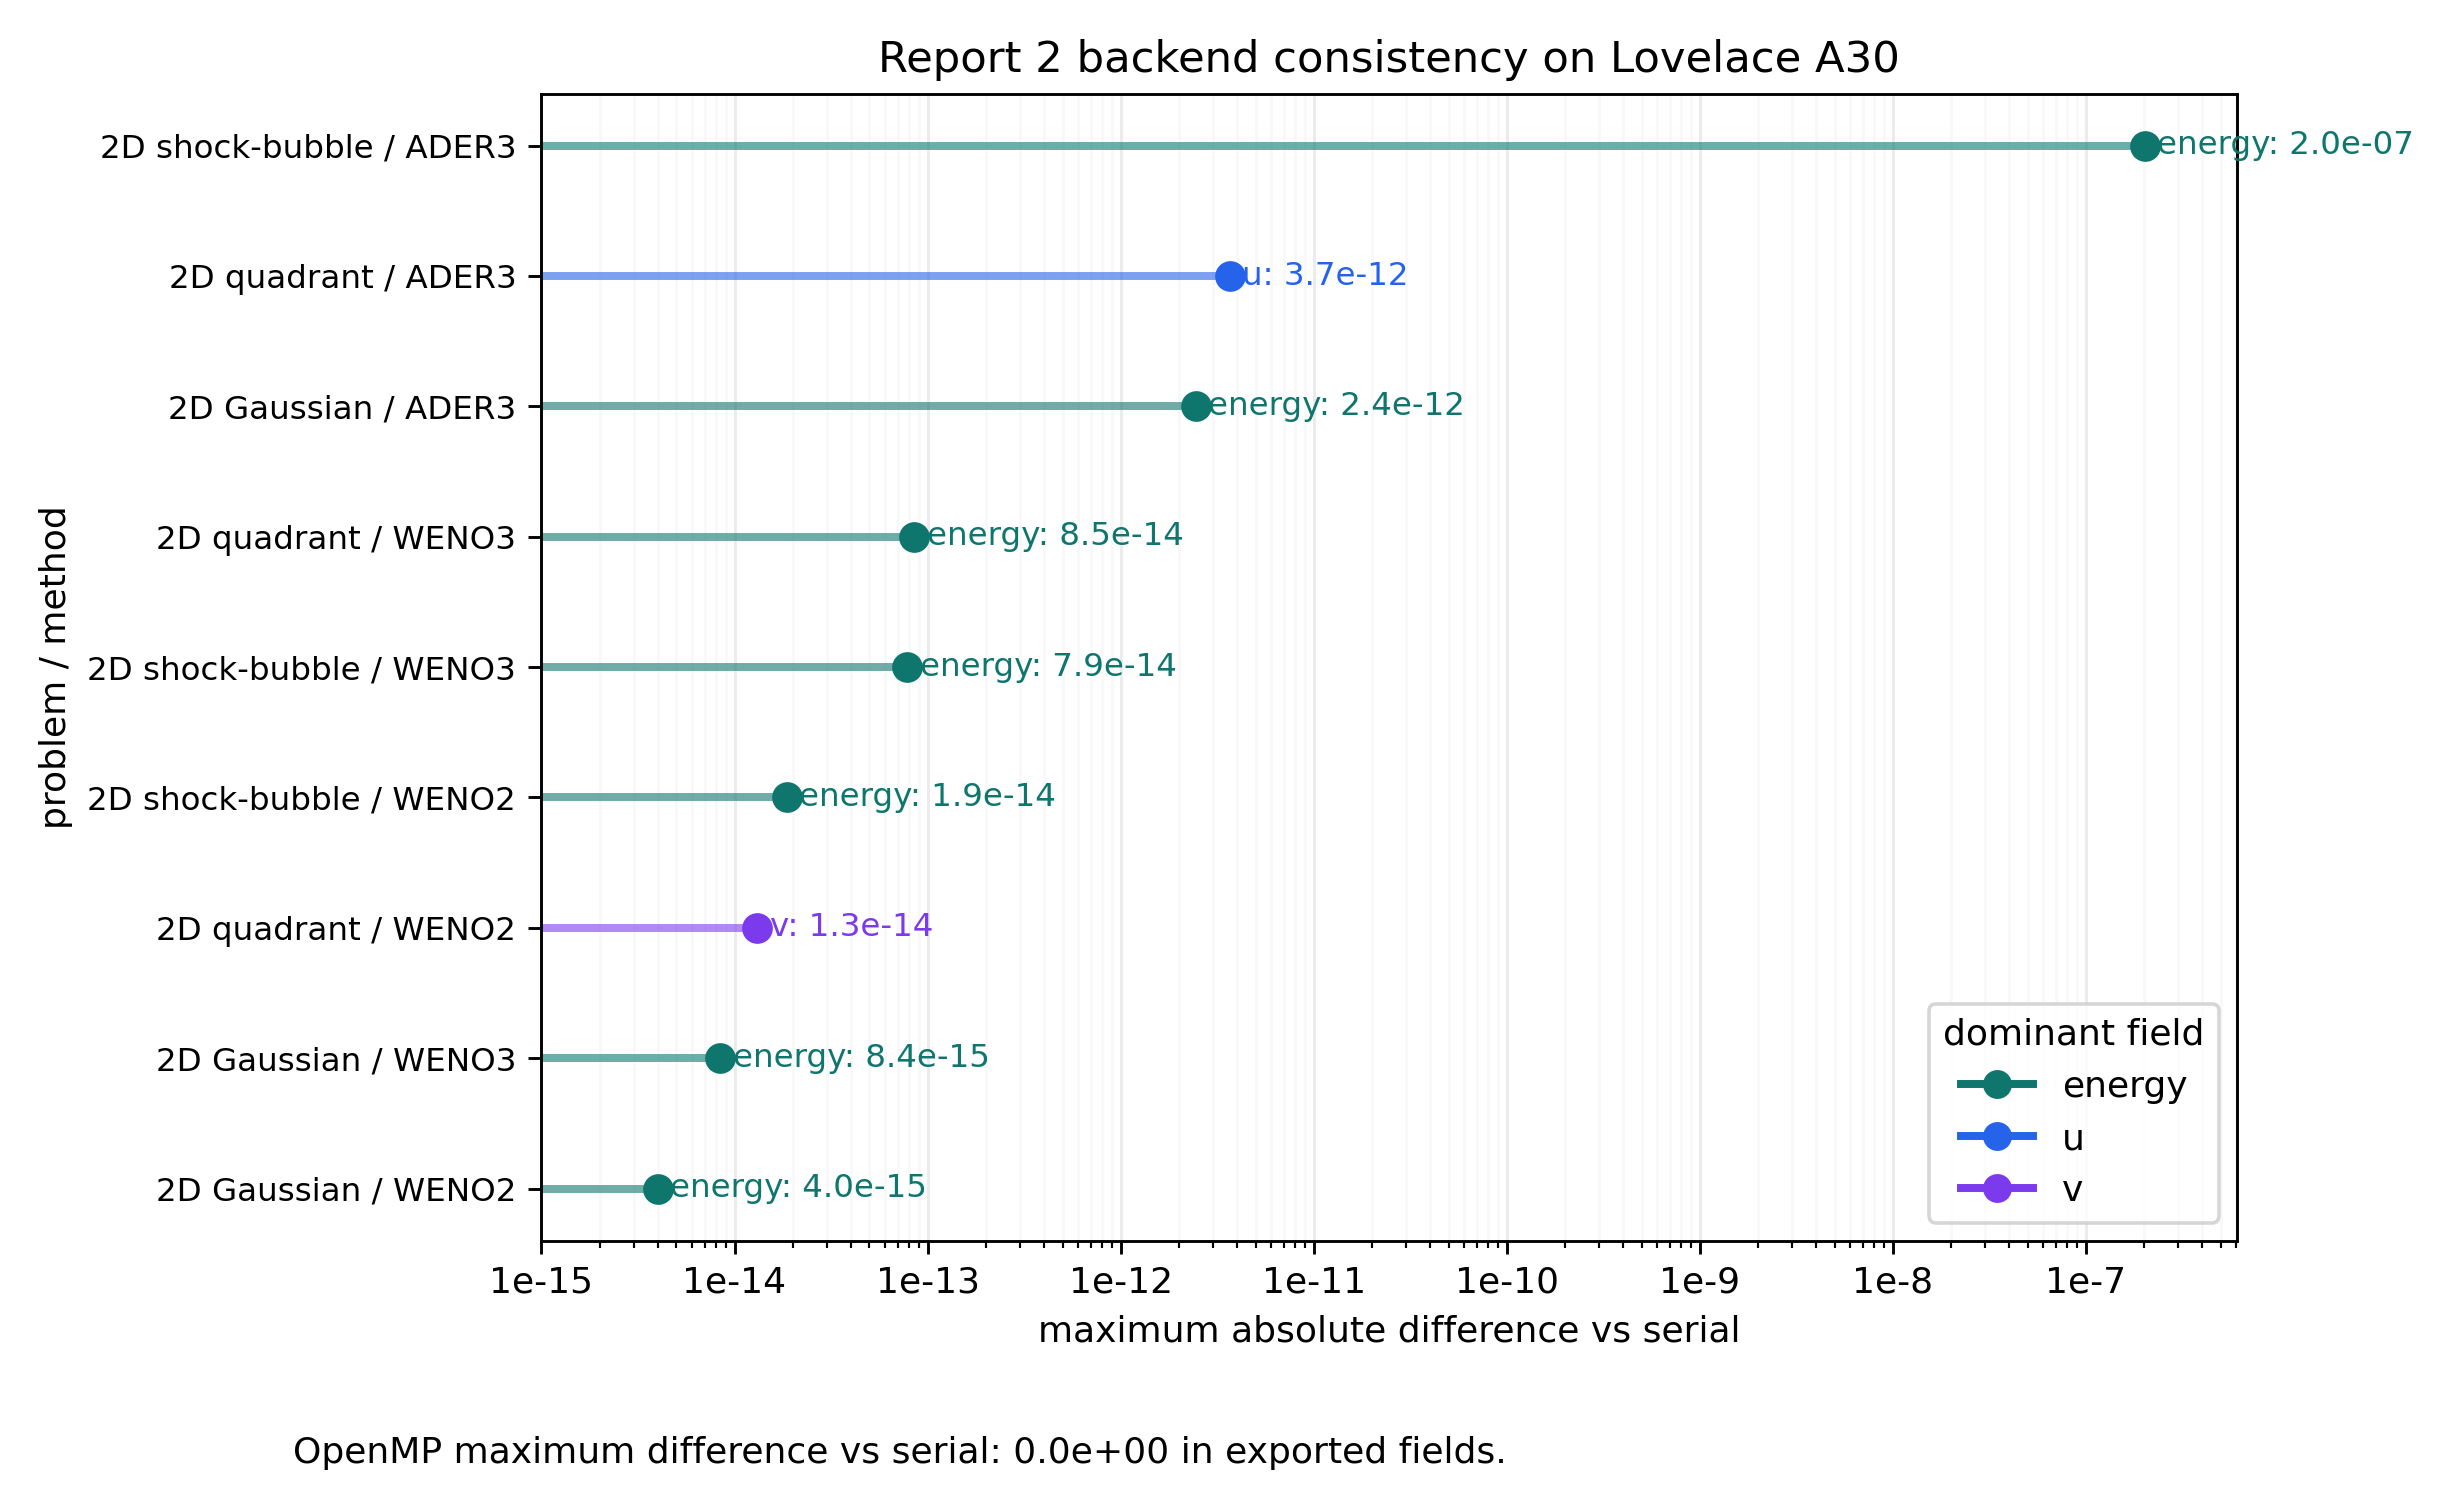
\includegraphics[width=0.88\textwidth]{backend_consistency_max_delta.png}
\caption{Largest CUDA--serial difference for each problem/method pair. OpenMP is omitted from the logarithmic axis because all stored OpenMP--serial differences are exactly zero.}
\label{fig:backend-consistency}
\end{figure}

\FloatBarrier
\section{Backend agreement and admissibility}

OpenMP matches serial exactly in all 45 stored fields. CUDA remains near roundoff for
both WENO methods and below \(4\times10^{-12}\) for smooth and quadrant ADER-3, far below
the discretisation errors in Chapter~\ref{chap:validation}. The sole larger entry is the
local shock--bubble ADER-3 energy difference of \(2.021\times10^{-7}\). Its alignment with
the moving interfaces identifies the nonlinear sensor/fallback branch as the cause rather
than a failed HLLC flux or displaced solution.

Table~\ref{tab:highres-positivity} provides the independent \(600^2\) admissibility check.
Every accepted field remains strictly positive. ADER-3 reaches the lowest shock--bubble
values but remains inside the physical domain.

\begin{table}[H]
\centering
\small
\begin{tabular}{llrr}
\toprule
Problem & Method & \(\min\rho\) & \(\min p\) \\
\midrule
Quadrant Riemann & WENO-2 & 0.137955 & 0.028944 \\
Quadrant Riemann & WENO-3 & 0.137936 & 0.028918 \\
Quadrant Riemann & ADER-3 & 0.137891 & 0.028987 \\
Shock--bubble & WENO-2 & 0.126797 & 0.999112 \\
Shock--bubble & WENO-3 & 0.127368 & 0.999683 \\
Shock--bubble & ADER-3 & 0.122012 & 0.968668 \\
\bottomrule
\end{tabular}
\caption{Minimum density and pressure in the accepted \(600\times600\) discontinuous HLLC fields.}
\label{tab:highres-positivity}
\end{table}

The three implementations therefore produce the same accepted physical solutions. The
following timings compare their execution cost rather than different numerical outcomes.

\FloatBarrier
